\chapter{WOman}
\cite{IncrLearnDailyRoutWorkflowSmartHomeEnvir} \cite{WoMan} WoMan è un sistema dichiarativo di process mining, in quanto capace di adottare rappresentazioni FOL (First-Order Logic). La FOL fornisce un'ottima espressività, utile per gestire domini complessi che coinvolgono una variabile quantità di oggetti con la possibilità che si verifichino diverse interazioni tra di essi; inoltre offre un unico framework in cui è possibile esprimere e combinare descrizioni di casi, modelli di processo e condizioni sulle attività, sia ai fini dell’apprendimento che dell’attuazione. 

Nella FOL, un predicato, scritto con la notazione usuale p/n, esprime una proprietà o una relazione p su n oggetti (chiamati i suoi argomenti). 

Un atomo è un predicato p/n applicato a n oggetti t1, ..., tn, scritto come p(t1, ..., tn); esso afferma che la proprietà o la relazione p si limita a quegli oggetti. Qui adotterò la rappresentazione classica della programmazione logica, in cui una virgola tra due atomi è indice della loro congiunzione, e le implicazioni possono essere espresse nella forma l0 :- l1, ..., lm, dove l0 è la conclusione e l1, ..., lm è la congiunzione delle premesse. Le sezioni seguenti mostrano come WoMan rappresenta e gestisce le informazioni necessarie per applicare le tecniche di process mining a un ambiente intelligente.

\section{Descrizione dei casi}
Il flusso di attività di un caso è espresso in WoMan come una congiunzione di atomi costruiti sui seguenti predicati:
\begin{itemize}
\item activity(S, T): al passo S viene eseguita l'attività T;
\item next(S, S'): il passo S segue il passo S'.
\end{itemize}

L'argomento T del predicato activity/2 è estrapolato da un insieme (fisso e dipendente dal contesto) di costanti che rappresentano le attività consentite. 

I passi, indicati da identificatori univoci, sono associati agli eventi e possono essere implementati come timestamp che indicano gli eventi associati. 

Il predicato next/2 consente di rappresentare esplicitamente le esecuzioni parallele nel flusso di attività; ciò evita la necessità di individuare il parallelismo tra le attività mediante considerazioni statistiche. 

Di fatti quest'approccio potrebbe risultare fuorviante e quindi indurre in errore il processo di apprendimento del flusso di lavoro. 

A partire dal formato a 6 tuple precedentemente introdotto, ogni attività può essere automaticamente tradotta in questo formato.

Ad esempio, l’attività campione per la routine del "pomeriggio" vista in \cite{IncrLearnDailyRoutWorkflowSmartHomeEnvir} sarebbe espressa come segue:

activity(s0,start), next(s0,s1), activity(s1,housekeeping), next(s1,s2), activity(s2,toilet),

next(s2,s3), activity(s3,relax), next(s3,s4), activity(s4,tea), next(s4,s5),

activity(s5,prepare\_snack), next(s5,s6), activity(s6,eat\_snack), next(s5,s7), activity(s7,radio),

next(s5,s8), activity(s8,magazine), next(s6,s9), next(s7,s9), next(s8,s9), activity(s9,stop).

Lo step s0 è associato all'attività "start", indicativa dell'inzio dell’attività. La prima attività ("housekeeping") è associata allo step s1. L'attività "toilet" è associata allo step s2 e ha una relazione "next" con "housekeeping" come attività più recentemente completata. Allo stesso modo, una sequenza di attività "relax", "tea" e "prepare\_snack" segue, portando allo step s5. Quindi, l'attività "eat\_snack", associata allo step s6, ha una relazione "next" con "prepare\_snack". Anche l'attività "radio", associata allo step s7, ha una relazione "next" con "prepare\_snack" ma non con "eat\_snack", che è ancora in esecuzione. Lo stesso vale per "magazine", associato allo step s8, che genera complessivamente tre attività concorrenti. Il caso termina al compimento delle tre attività, come indicato dalle relazioni "next" tra i rispettivi passi e lo step s9, associato all'attività fittizia "stop" che indica la fine del caso.

Utilizzando ulteriori predicati dipendenti dal dominio, è possibile aggiungere scorrevolmente ulteriori informazioni di contesto e relazioni relative agli step e alle attività alla descrizione, sostando all'interno del framework FOL. 

Mentre i predicati activity/2 e next/2 sono riservati, è possibile definire e utilizzare qualsiasi altro predicato da parte dell'ingegnere della conoscenza, responsabile di garantire la coerenza nella definizione e nell'uso di questi predicati, per esprimere informazioni di contesto senza richiedere modifiche al sistema; ciò consente un'applicazione generale dell'approccio nei più svariati domini e compiti. 

Consideriamo, ad esempio, l'estensione seguente del nostro caso di esempio, la quale esprime le relative informazioni di contesto:

early\_afternoon(s1), sunny(s1), air\_conditioning\_on(s1),

early\_afternoon(s2), sunny(s2), short\_duration(s2), short\_interval(s2,s3),

early\_afternoon(s3), sunny(s3), air\_conditioning\_on(s3), long\_duration(s3),

mid\_afternoon(s4), cloudy(s4), humidity\_high(s4),

mid\_afternoon(s5), rainy(s5), microwave\_on(s5),

late\_afternoon(s6), rainy(s6),

late\_afternoon(s7), rainy(s7), radio\_on(s7), news(s2,n’), about(n’,s), sports(s), bad(n’),

late\_afternoon(s8), rainy(s8),

Si desume che fosse presto, il tempo fosse soleggiato e l'aria condizionata accesa mentre l'utente svolgeva l'attività di "housekeeping’’. Era presto e soleggiato, ma l'aria condizionata era spenta anche quando è andato in bagno, dove è rimasto per breve tempo. Dopo un breve intervallo ha iniziato a rilassarsi, con l'aria condizionata accesa e il tempo ancora soleggiato. Il relax è durato a lungo e quando l'utente ha preso il tè nel pomeriggio il tempo era nuvoloso e umido. Ha iniziato a piovere mentre stava preparando uno spuntino nel forno a microonde, dopodiché, nel tardo pomeriggio, la pioggia non accennava a fermarsi e la radio ha dato notizie negative sullo sport.
\section{Learning Workflow Structure and Weights}
Nel sistema WoMan, una struttura di flusso di lavoro è descritta come una congiunzione di atomi costruiti sui seguenti predicati:
\begin{itemize}
\item task(t,C): il task t si verifica nei casi C;
\item transition(I,O,p,C): la transizione p, che si verifica nei casi C, consiste nel terminare tutti i task in I (che devono essere in esecuzione) e avviare l'esecuzione di nuove istanze di tutti i task in O.
\end{itemize}

L'argomento C dei due predicati è uno storico che riporta gli identificatori dei casi in cui si è incontrato il task/transizione.

È un multi insieme perché un task/transizione può verificarsi più volte nello stesso caso; esso può essere sfruttato per calcolare statistiche sul loro utilizzo e per decrementare la ridondanza, imponendo che la sequenza di transizioni osservata durante il funzionamento del modello si sia verificata almeno in un caso di addestramento. 

Un modello è espresso come un insieme (da interpretare come una congiunzione) di atomi costruiti su questi predicati e viene costruito come riportato nell'Algoritmo seguente:

\begin{figure}
    \begin{center}    
        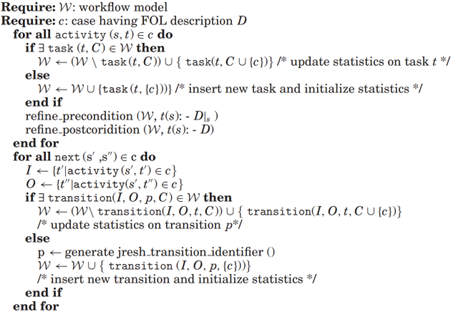
\includegraphics[width=0.9\linewidth]{images/53.png}
    \end{center}
\end{figure}
 

WoMan funziona nel seguente modo: preleva un nuovo caso di addestramento c e lo utilizza per aggiornare un modello di flusso di lavoro esistente, se presente, o per costruire un nuovo modello dal principio, se è il primo caso considerato. Indi, è completamente incrementale. Durante la gestione del caso, crea/aggiorna prima i task nel modello per poi creare/aggiornare le transizioni. 

Per quanto riguarda i task, per ogni atomo $activity(s, t)$ in $c$, se un atomo $task(t, C)$ è già presente nel modello corrente, viene sostituito con $task(t, C \cup {c})$, altrimenti viene aggiunto un nuovo atomo $task(t, {c})$ al modello corrente. Per quanto riguarda le transizioni, ogni atomo $next(s, s')$ in $c$ deve appartenere a una transizione con $I$ e $O$ tali che $s \in I$ e $s' \in O$.

Pertanto, devi selezionare ed eliminare da $c$ gli altri atomi $next/2$ che si riferiscono alla stessa transizione, ottenendo $I$ e $O$, e quindi sostituire (se presente) l'atomo $transition(I, O, p, C)$ con $transition(I, O, p, C \cup {c})$, o creare un nuovo atomo $transition(I, O, p, {c})$, dove $p$ è un nuovo identificatore di transizione, nel caso in cui non esista.

Per quanto riguarda la selezione degli atomi next/2, molti atomi next(s, si) indicano che l'esecuzione del task associato allo step s è seguita dall'esecuzione parallela dei task associati agli step si, quindi i task associati ai si devono essere inclusi in O. 

Allo stesso modo, molti atomi next(sj, s) indicano che l'esecuzione di vari task paralleli associati agli step sj converge nell'esecuzione del task associato allo step s, quindi i task associati ai sj devono essere inclusi in I.

Per ciascun si (rispettivamente, sj), la stessa procedura deve essere iterata per trovare altri atomi next(sh, si) (next(sj, sk), rispettivamente), e così via fino alla convergenza. 

Ciò accade quando è necessario interrompere più task di input paralleli e/o avviare più task di output nello stesso passaggio, una situazione che richiederebbe modelli complessi per essere rappresentati utilizzando le reti di Petri.

Esecuzioni alternative possono emergere dall'analisi di diversi casi che selezionano diverse opzioni di routing nello schema di flusso di lavoro, rappresentate in seguito da diversi atomi transition/2. La rappresentazione proposta implica una gestione fluida e naturale dei casi complessi o problematici che coinvolgono nodi di task invisibili o duplicati, che solitamente sono problematici da rappresentare nelle reti di Petri e da apprendere con le altre tecniche disponibili in letteratura. 

Infatti, diversi nodi transition/2 possono combinare un dato task in modi diversi con altri task o ignorare un task quando non è obbligatorio per un passaggio specifico. 

Nel complesso, i modelli appresi da WoMan sono un superset stretto di quelli che possono essere espressi dalle reti di Petri; tuttavia, quando un modello WoMan rientra nell'intervallo esprimibile dalle reti di Petri, può essere facilmente e automaticamente tradotto in tale formalismo.

WoMan ha la facoltà di gestire anche il rumore; di fatti, le probabilità delle transizioni sono proporzionali al numero di casi in cui si sono effettivamente verificate, ovvero alla cardinalità del multiset associato di casi: quando viene elaborato un nuovo caso di addestramento, l'aggiornamento di questi multisets comporta anche l'aggiornamento dei pesi come effetto collaterale. 

Pertanto, sebbene i casi rumorosi siano effettivamente incorporati nel modello, imporre una tolleranza al rumore $N \in [0,1]$ significa semplicemente ignorare tutte le transizioni la cui frequenza è inferiore a $N$.

WoMan apprende dagli esempi costituiti da descrizioni complete dei casi, ma è in grado di applicare il modello appreso in modo progressivo finché vengono generati gli eventi di log. La procedura, la cui versione formale dell'algoritmo è riportata in \cite{WoMan}, può essere riassunta come segue: le 6-tuple delineanti gli eventi che si verificano nell'ambiente vengono inviate al sistema man mano che vengono generate; il sistema le sfrutta per navigare nel modello, tenendo traccia in ogni momento delle attività ancora in corso. 

Quando si verifica un evento “begin activity”, il sistema verifica se una transizione nel modello consente di passare dallo stato corrente alla nuova attività; quando invece si verifica un evento “end activity”, il sistema aggiorna lo stato corrente chiudendo quella attività. 

Sulla base di questi controlli, il sistema può rispondere immediatamente in corso di routine , restituendo per ogni evento uno dei seguenti esiti: "ok" (se l'evento è conforme al modello nello stato corrente del flusso di lavoro), "warning" (se l'evento non è conforme al modello nello stato corrente del flusso di lavoro, ma potrebbe comunque indicare un nuovo ramo della routine da poter utilizzare per perfezionare il modelloa caso concluso), "errore" (se l'evento non è accettabile nello stato corrente del flusso di lavoro - ad esempio, terminare un'attività che non era mai iniziata o chiudere il caso mentre alcune attività sono ancora in corso). 

Nel caso di un warning, può specificare se il problema è dovuto a un'attività o transizione inaspettata, consentendo all'ambiente intelligente di intraprendere le opportune contromisure e di mantenere statistiche sui problemi che si sono verificati durante l'esecuzione del flusso di lavoro/routine. 

Ciò assicura che WoMan venga, in teoria, applicato in tempo reale e che possa verificare progressivamente, finché gli eventi e le attività si concludono, la loro conformità al modello della routine. 

Il sistema può gestire più routine non separate temporalmente, alimentando gli eventi e le attività che si verificano a tutti i modelli di routine attivi. Pertanto, il sistema non distingue a priori quali eventi/attività appartengono a quale routine, ma ogni modello può sfruttare o ignorare questi eventi/attività secondo necessità. 

Le routine sono considerate indipendenti l'una dall'altra, indi per cui il sistema non è in grado di imporre alcun tipo di sincronizzazione tra di loro; se tale sincronizzazione è significativa, è necessario apprendere una routine composta che coinvolga esplicitamente tutte le attività delle singole routine. 

Anche nella fase di apprendimento, è possibile gestire più routine contemporaneamente, ma in questo caso è necessaria la presenza di un modo per il sistema di capire quali attività devono essere alimentate a quale modello.

\section{Realizzazione file per l’osservazione e la predizione dei mood attraverso il sistema WOman}

Per la realizzazione di questi file ho proseguito in questo modo:
\begin{itemize}
    \item Ho in inizialmente ridotto la pull di mood da poter analizzare in quanto solo 2 confused, engaged, bored e frustrated sono presenti all’interno del dataset DAiSEE \cite{DAiSEE} che, a differenza dello student-engagement-dataset \cite{StudEngagDataset}, il quale presenta solo immagini, è composto solo da video.
    \item Successivamente ho scomposto il video utilizzando sempre il metodo \mintinline[bgcolor=bg]{python}{detector.detect_video(videoPath)}; come è possibile notare, il parametro \mintinline[bgcolor=bg]{python}{skip_frames} non è valorizzato. Quando questo parametro non è valorizzato il valore diventa \mintinline[bgcolor=bg]{python}{None}, ovvero non viene saltato nessuno dei frame del video.
    Effettuo quindi un’analisi su ognuno dei frame dei video analizzati, rielaboro l’output di queste ed ottengo l’input per il sistema WOman.
    \item Ognuna delle linee dei file di input prodotti è così strutturata: (T, E, W, P, A, O), dove: 
    \begin{itemize}
        \item T è suddiviso in \colorbox{yellow}{frame in cui avviene l'attivazione della singola action} \colorbox{yellow}{units} e \colorbox{green}{numero di utilizzo di questo frame},
        \item \colorbox{red}{E} è il tipo di evento che sta avvenendo in quel frame (begin of process, end of process, begin of activity, end of activity), 
        \item \colorbox{blue}{W} è il mood del video relativo,
        \item \colorbox{purple}{P} è il video che sto adoperando per l’analisi, 
        \item \colorbox{brown}{A} è l’Action Unit che è stata attivata o che si è spenta,
        \item \colorbox{pink}{O} è il numero progressivo relativo a quante volte la singola Action Unit si è accesa e spenta (il numero progressivo di occorrenze di A in P) 
    \end{itemize}
\end{itemize}

Genero quindi, ad esempio, stringhe come queste:
\begin{minted}[escapeinside=||, bgcolor=bg]{python}
entry(|\colorbox{yellow}{000}\colorbox{green}{00}|,|\colorbox{red}{begin\_of\_process}|,|\colorbox{blue}{confused}|,|\colorbox{purple}{video987736015}|,|\colorbox{brown}{start}|,|\colorbox{pink}{1}|).
entry(00100,begin_of_activity,confused,video987736015,au02,1).
entry(00101,begin_of_activity,confused,video987736015,au24,1).
entry(00200,end_of_activity,confused,video987736015,au02,1).
entry(00201,begin_of_activity,confused,video987736015,au14,1).
entry(00202,begin_of_activity,confused,video987736015,au23,1).
entry(00203,end_of_activity,confused,video987736015,au24,1).
entry(00300,begin_of_activity,confused,video987736015,au07,1).
entry(00301,end_of_activity,confused,video987736015,au14,1).
entry(00302,end_of_activity,confused,video987736015,au23,1).
entry(00303,begin_of_activity,confused,video987736015,au24,2).
\end{minted}

Una volta realizzati questi file li ho consegnati al professore di modo che potesse fornirli al sistema.

Ho analizzato 50 file per ognuna delle label all’interno di DAiSEE e il dataset risultato, in formato json, è così strutturato:
\begin{minted}[bgcolor=bg]{json}
[
    {
        "AU01": {"valore frame per frame"},
        "AU02": {"valore frame per frame"},
        "…": "tutte le Action Units utilizzate da py-feat e 
                precedentemente citate"
        "AU28": {"valore frame per frame"},
        "AU43": {"valore frame per frame"},
        "input": {"valore frame per frame"},
        "label": "la label relativa al video"
    },
    "…":{"gli altri valori"}
]
\end{minted}

La label per ognuno dei video è stata estratta, attraverso il file “AllLabels” contenuto all’interno del dataset DAiSEE; il file è strutturato come segue:
\begin{minted}[bgcolor=bg]{python}
ClipID,Boredom,Engagement,Confusion,Frustration 
1100011002.avi,0,2,0,0
1100011003.avi,0,2,0,0
1100011004.avi,0,3,0,0
1100011005.avi,0,3,0,0
1100011006.avi,0,3,0,0
1100011007.avi,1,2,0,0
1100011008.avi,0,3,0,0
1100011009.avi,0,2,1,0
1100011010.avi,0,3,0,0
1100011011.avi,0,3,0,0
\end{minted}
È un file con estensione csv che presenta cinque colonne:
\begin{itemize}
\item l’identificativo del video, riportato poi anche nella colonna input del mio dataset derivato,
\item un valore fra 0 e 3 per la label bored,
\item un valore fra 0 e 3 per la label engaged,
\item un valore fra 0 e 3 per la label confused,
\item un valore fra 0 e 3 per la label frustrated,
\end{itemize} 
Hai fini del mio studio ho deciso di assegnare una singola label ad ognuno dei video in base al valore più alto fra quelli presenti.

Il numero di 50 file per ognuno dei mood è stato scelto in quanto era il numero migliore per quanto riguarda il rapporto numero di dati da utilizzare e tempo per generare questi dati:

ogni video di quelli presenti all’interno del dataset \cite{DAiSEE} sono lunghi fra i 5 e 6 secondi, che diventano quindi fra i 270 e i 300 frame da analizzare; effettuando un test sommario sulla durata dell’analisi per un video di 300 frames ci sono voluti 192.60754 secondi, sostituendo la media del numero di frame nei video (285) a quelli del video analizzato ottengo un tempo di analisi medio di 182,97716 secondi.

Moltiplicando questo valore per 200 ottengo 10,16539 ore alle quali vanno aggiunte le ore per scrivere su disco ognuna delle analisi e per generare i file con le entry riportate sopra. C’è poi da considerare la questione di surriscaldamento e relativo thermal throttling; il numero sopra riportato è stato ottenuto dall’esecuzione dell’analisi di un singolo video, è ragionevole pensare che, dopo aver raggiunto una temperatura abbastanza alta, il tempo di esecuzione delle singole analisi aumenti. 

Viene da sé che non è sostenibile, sia per quanto riguarda il tempo da dedicare a questa operazione sia a livello di costi, l’analisi di molti altri video, come si è poi rivelato necessario e che, da quanto si evince da \cite{WOman} invece, non avrebbero dovuto essere necessari. 

\section{Generazione dei modelli workflow attraverso WOman}
Una volta generati i file con le entry ho fornito questi al professore che ha eseguito il framework dando in input i file risultanti per tutti i video di ognuno dei video uniti in sequenza.

Mi sono stati forniti due file per ognuno dei mood:
\begin{itemize}
\item il primo contiene il numero di task e di transition per ognuno dei casi (o activity) analizzati dal sistema che stanno a segnalare il numero di nuove task e di transizioni effettuate ad ogni nuovo video analizzato dal sistema per lo specifico workflow (o mood).
\item nel secondo è presente invece il modello generato per ogni mood
\end{itemize}

Riporto qui i grafici generati per il primo tipo di tipo di file:
\newpage
\begin{figure}  
    \centering
    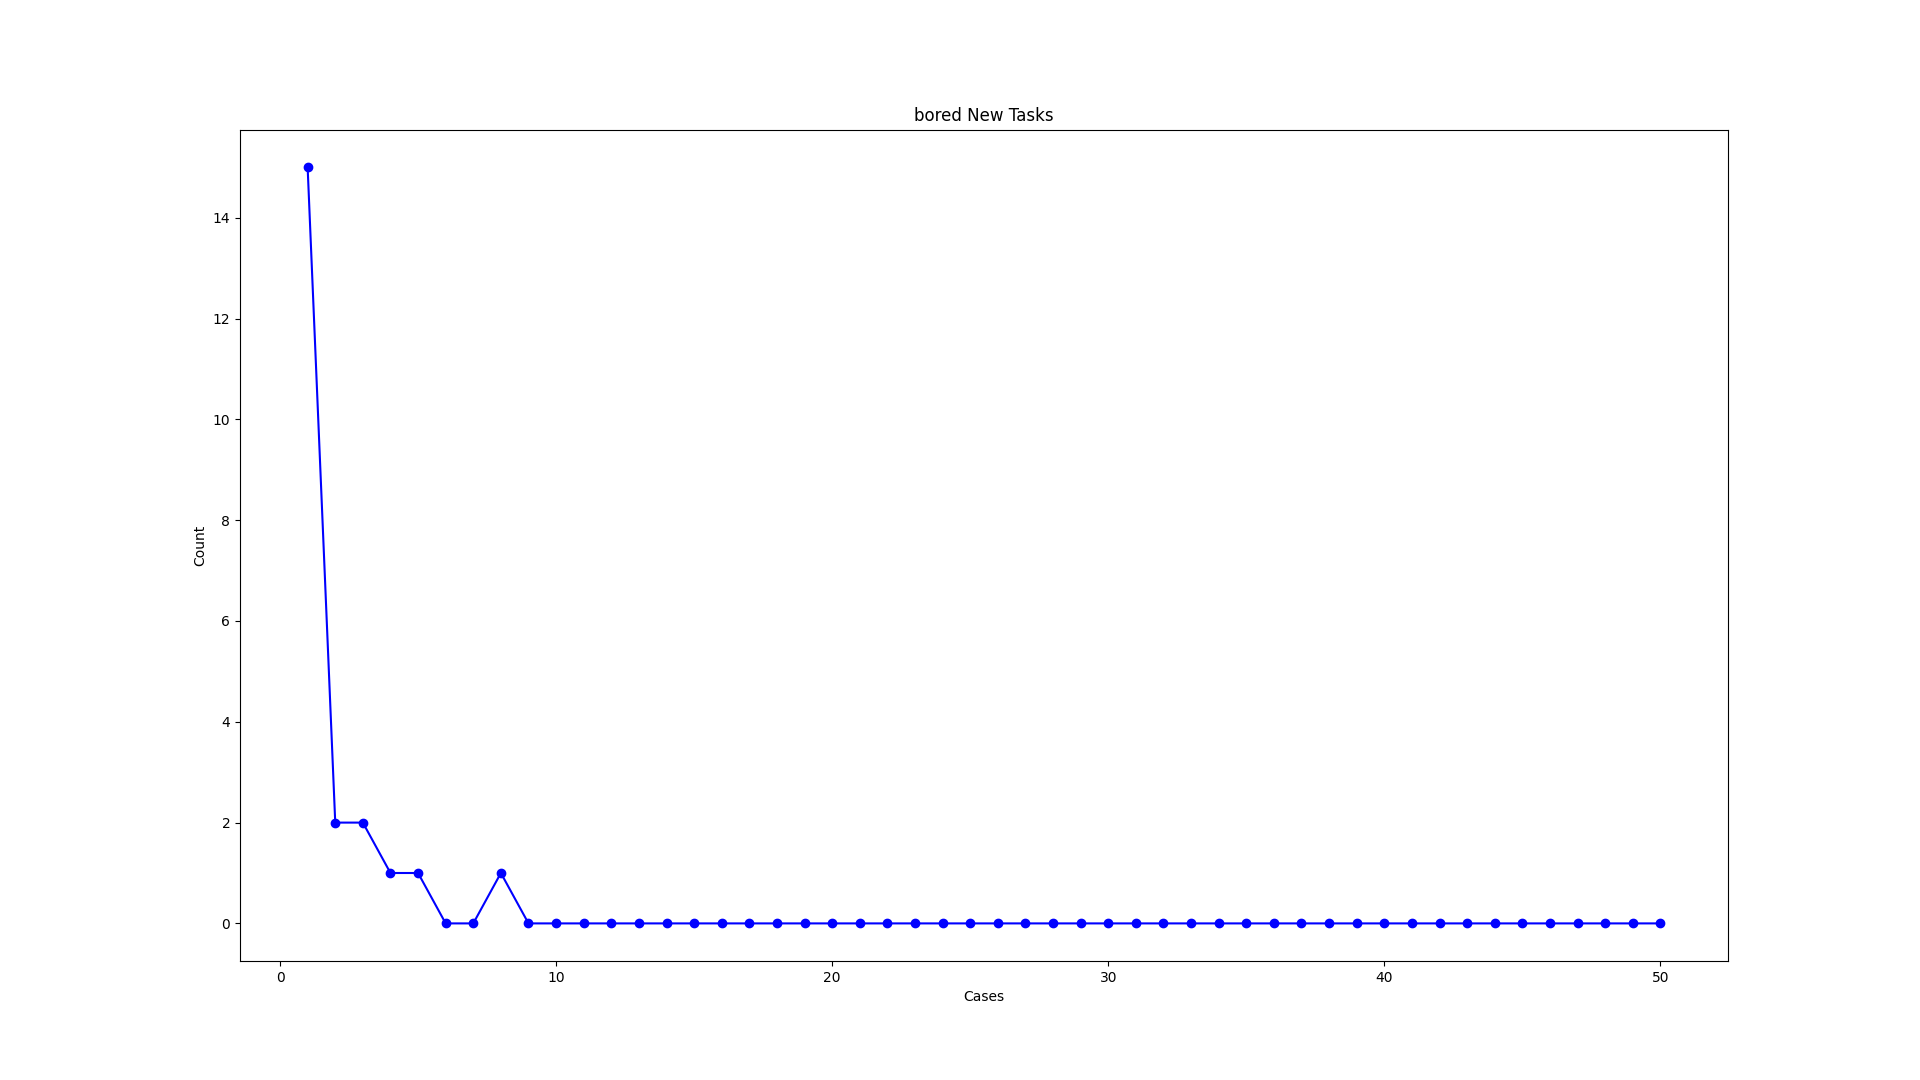
\includegraphics[width=1\linewidth]{images/bored New Tasks.png}
\end{figure}
\begin{figure}
    \centering   
    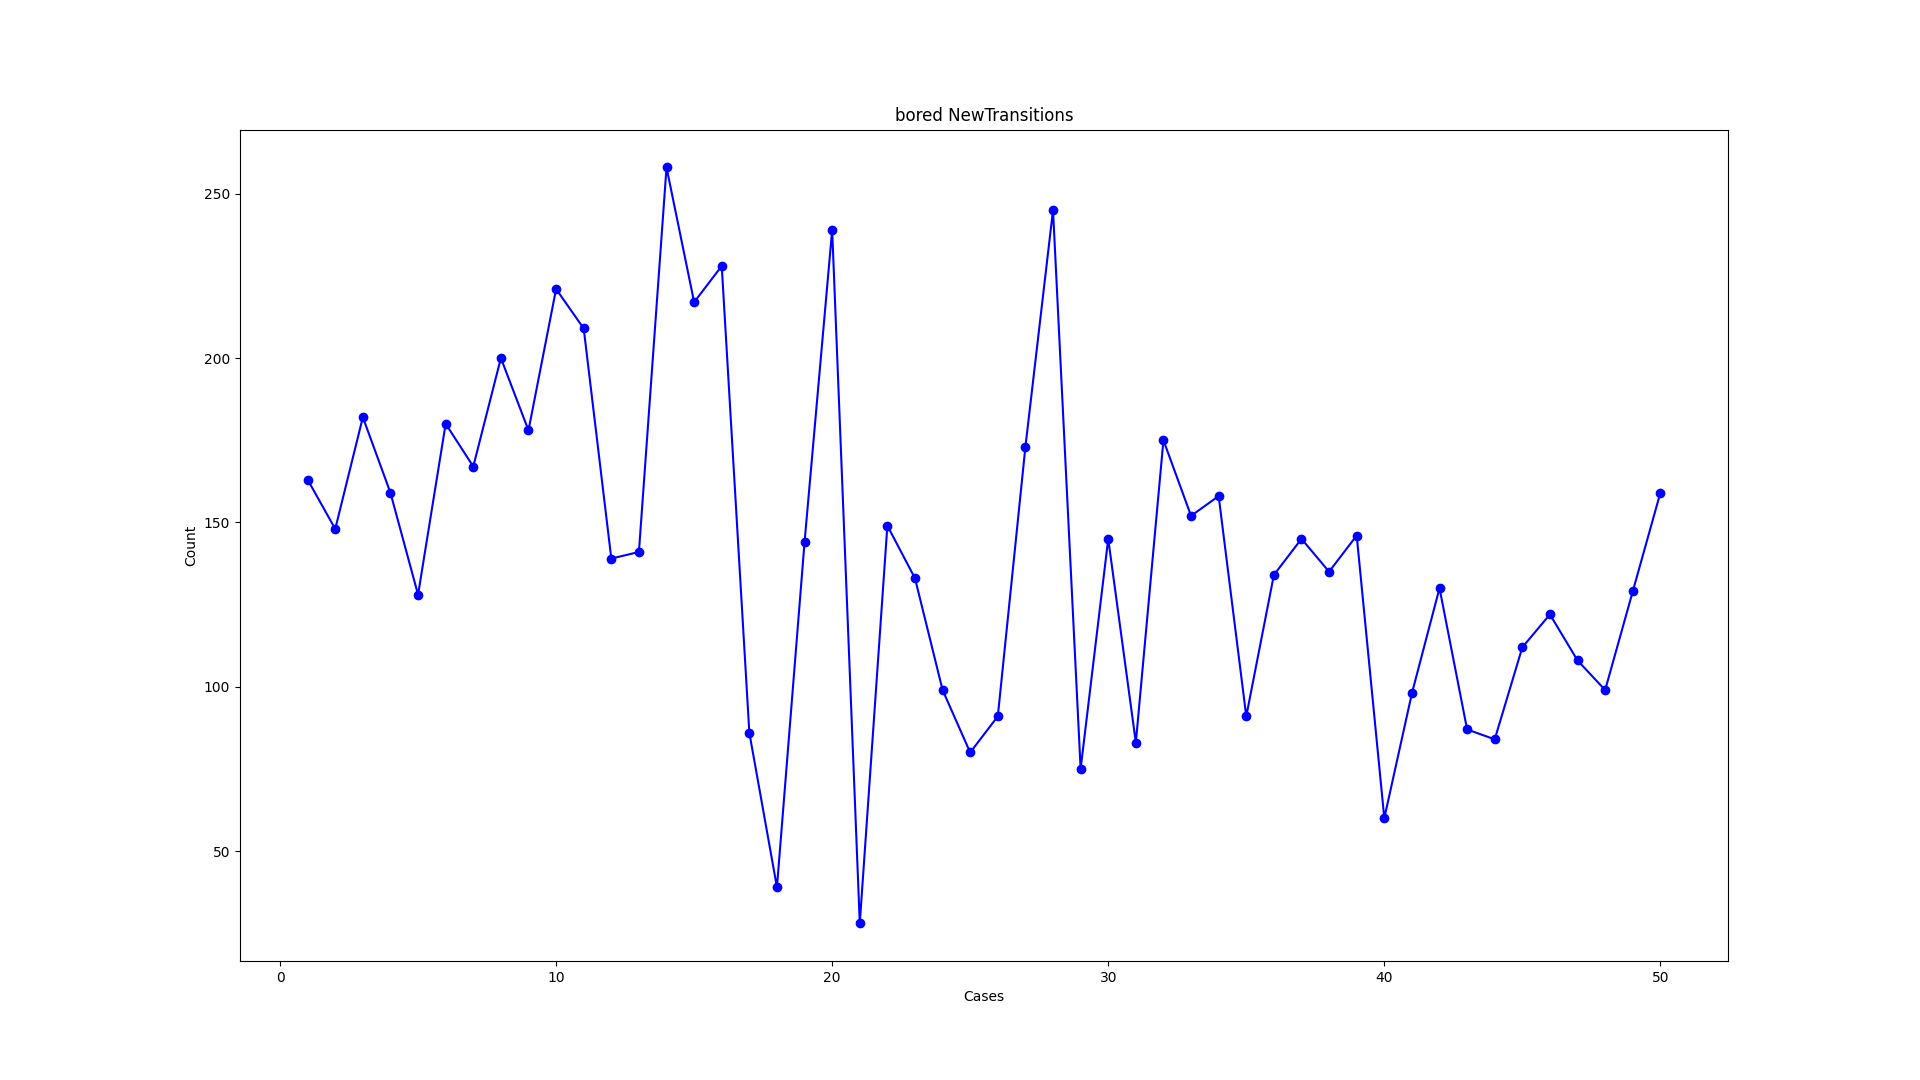
\includegraphics[width=1\linewidth]{images/bored NewTransitions.png}
\end{figure}\clearpage
\begin{figure}
    \centering   
    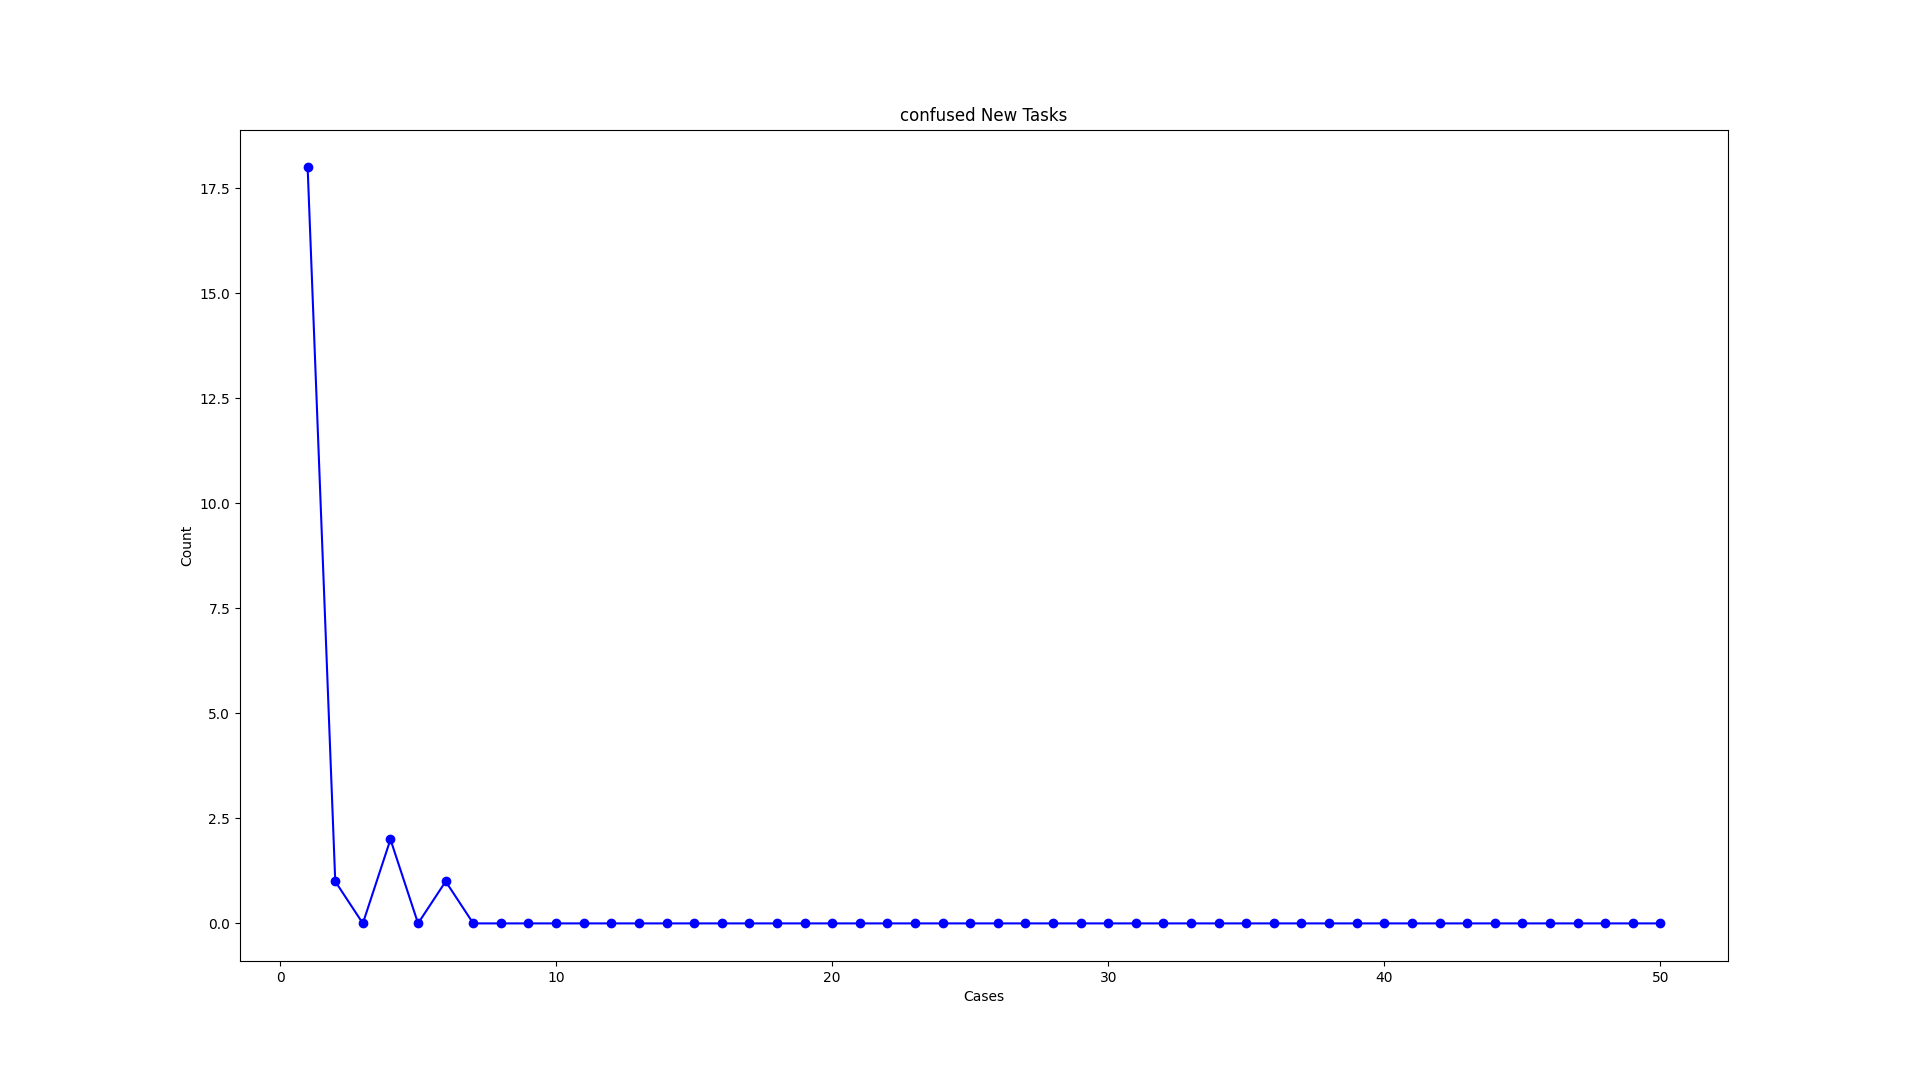
\includegraphics[width=1\linewidth]{images/confused New Tasks.png}
\end{figure}
\begin{figure}
    \centering   
    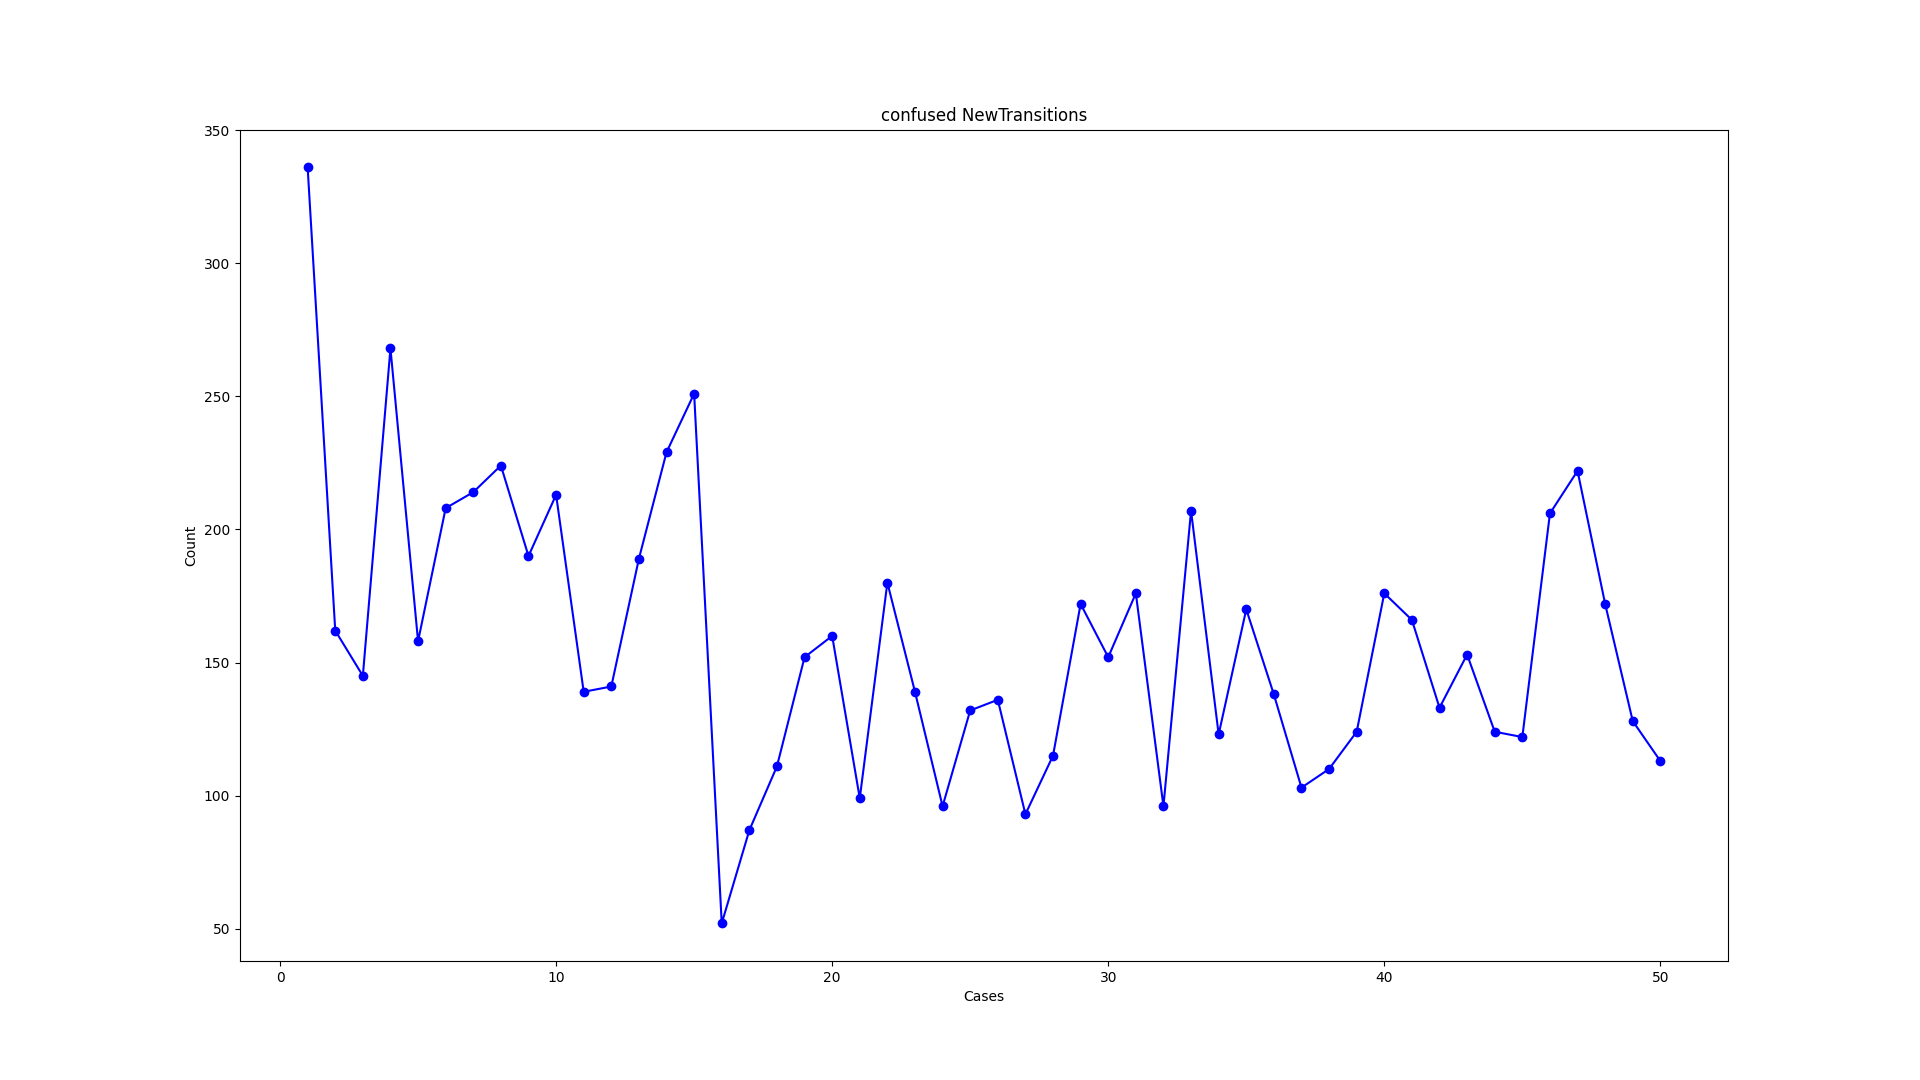
\includegraphics[width=1\linewidth]{images/confused NewTransitions.png}
\end{figure}\clearpage
\begin{figure}
    \centering   
    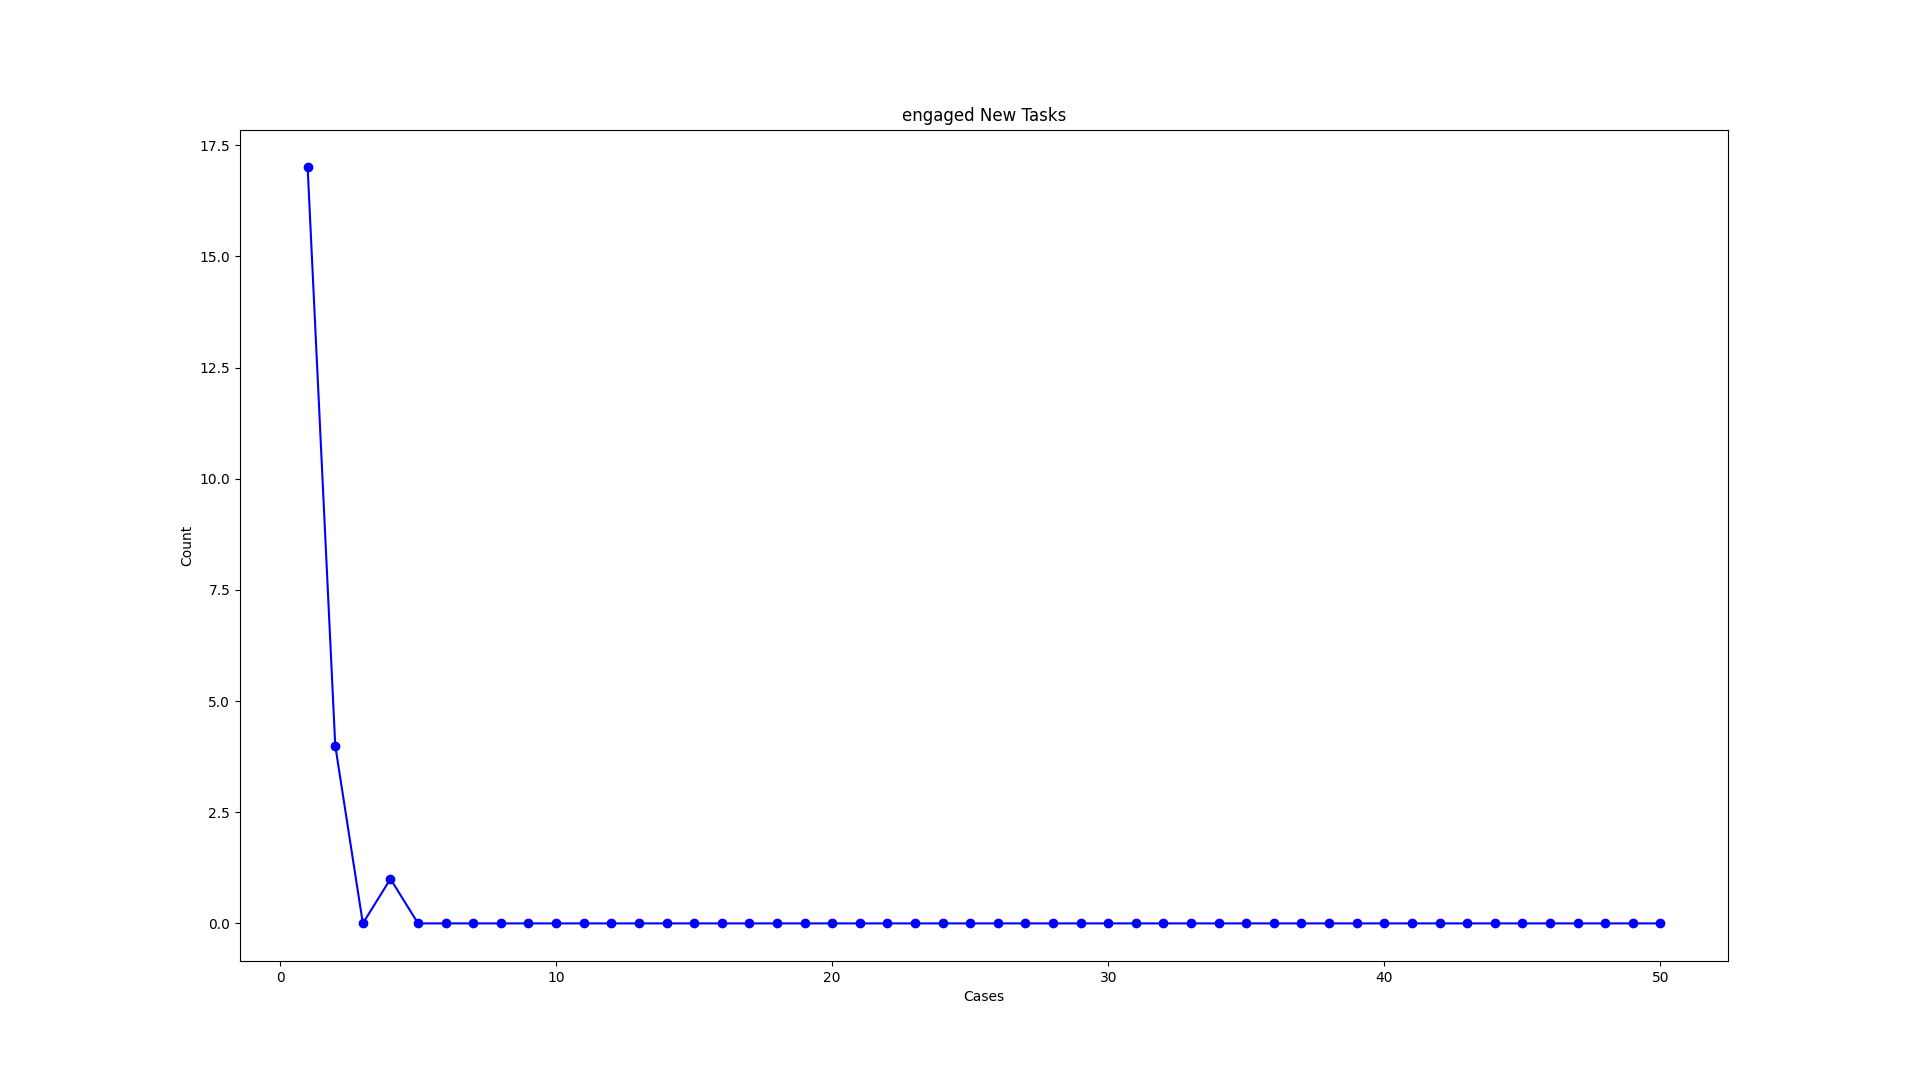
\includegraphics[width=1\linewidth]{images/engaged New Tasks.png}
\end{figure}
\begin{figure}
    \centering   
    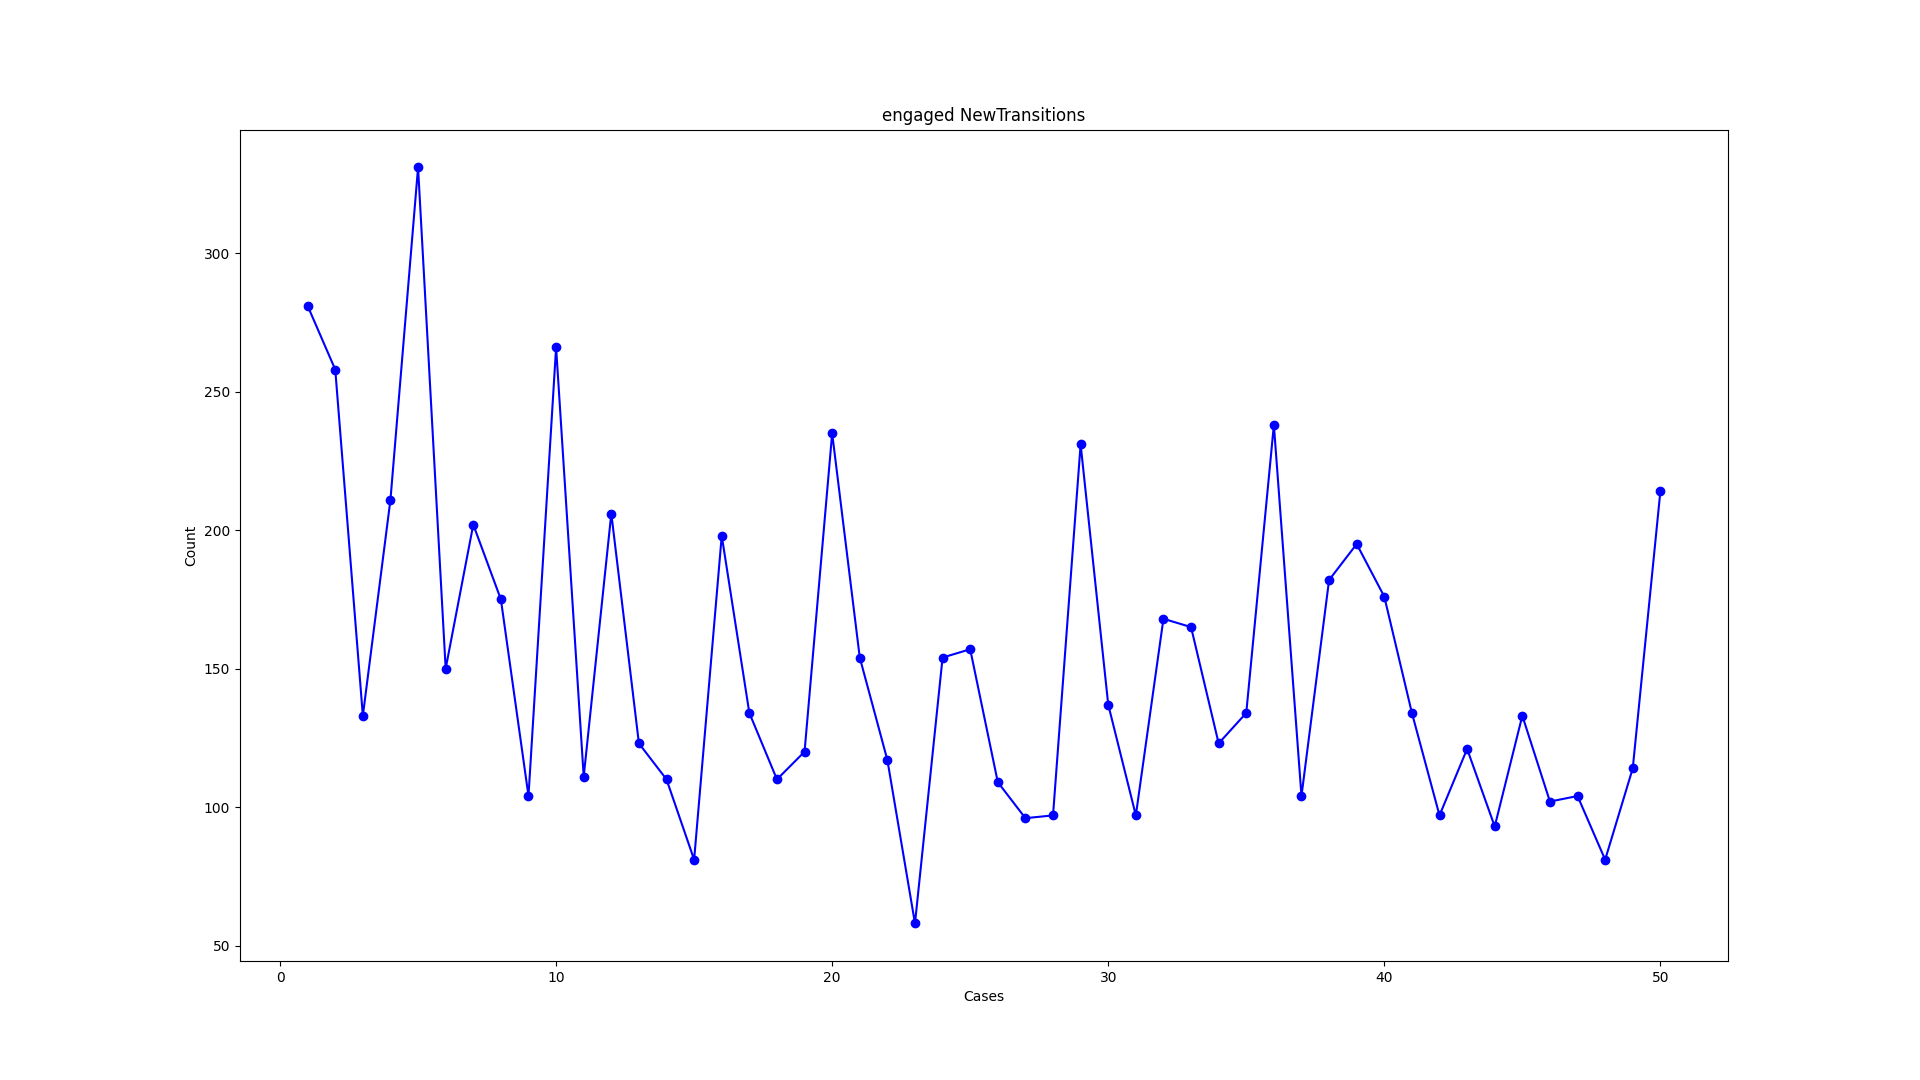
\includegraphics[width=1\linewidth]{images/engaged NewTransitions.png}
\end{figure}\clearpage
\begin{figure}
    \centering   
    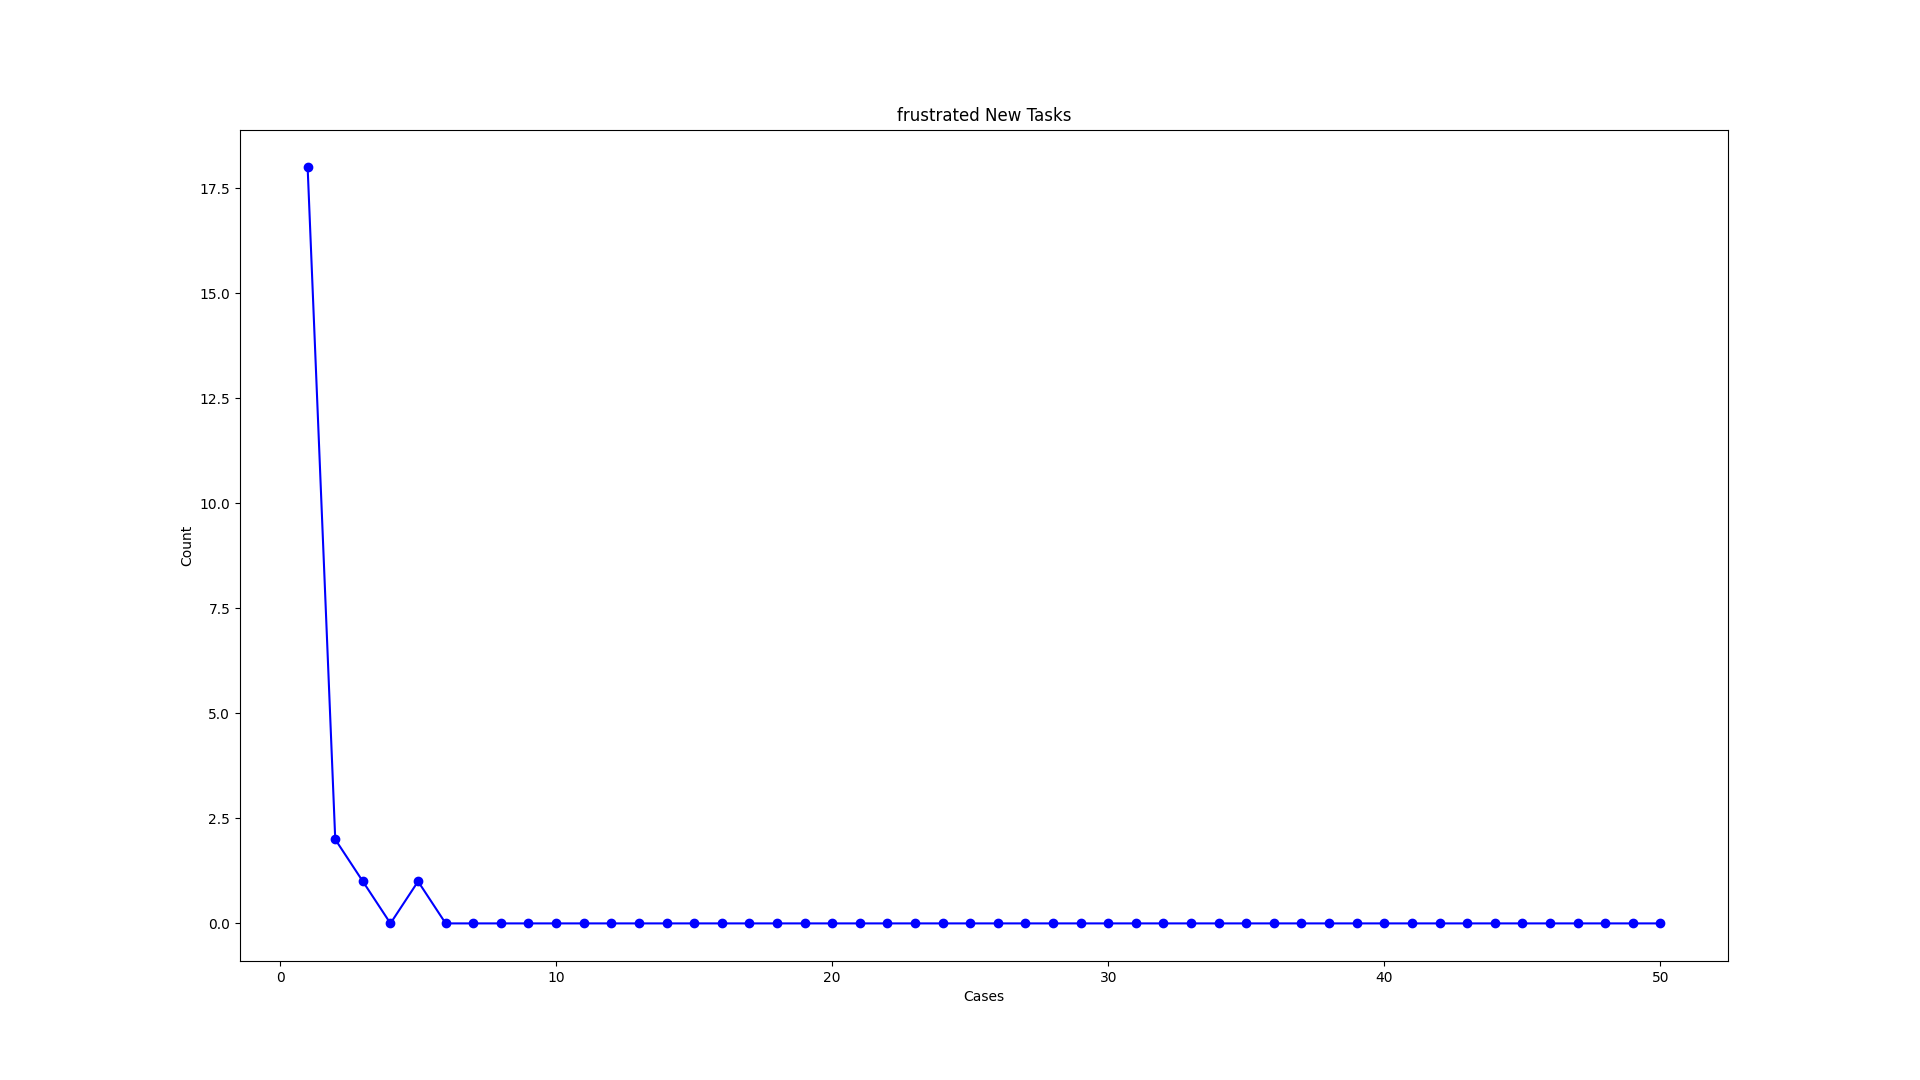
\includegraphics[width=1\linewidth]{images/frustrated New Tasks.png}
\end{figure}
\begin{figure}
    \centering   
    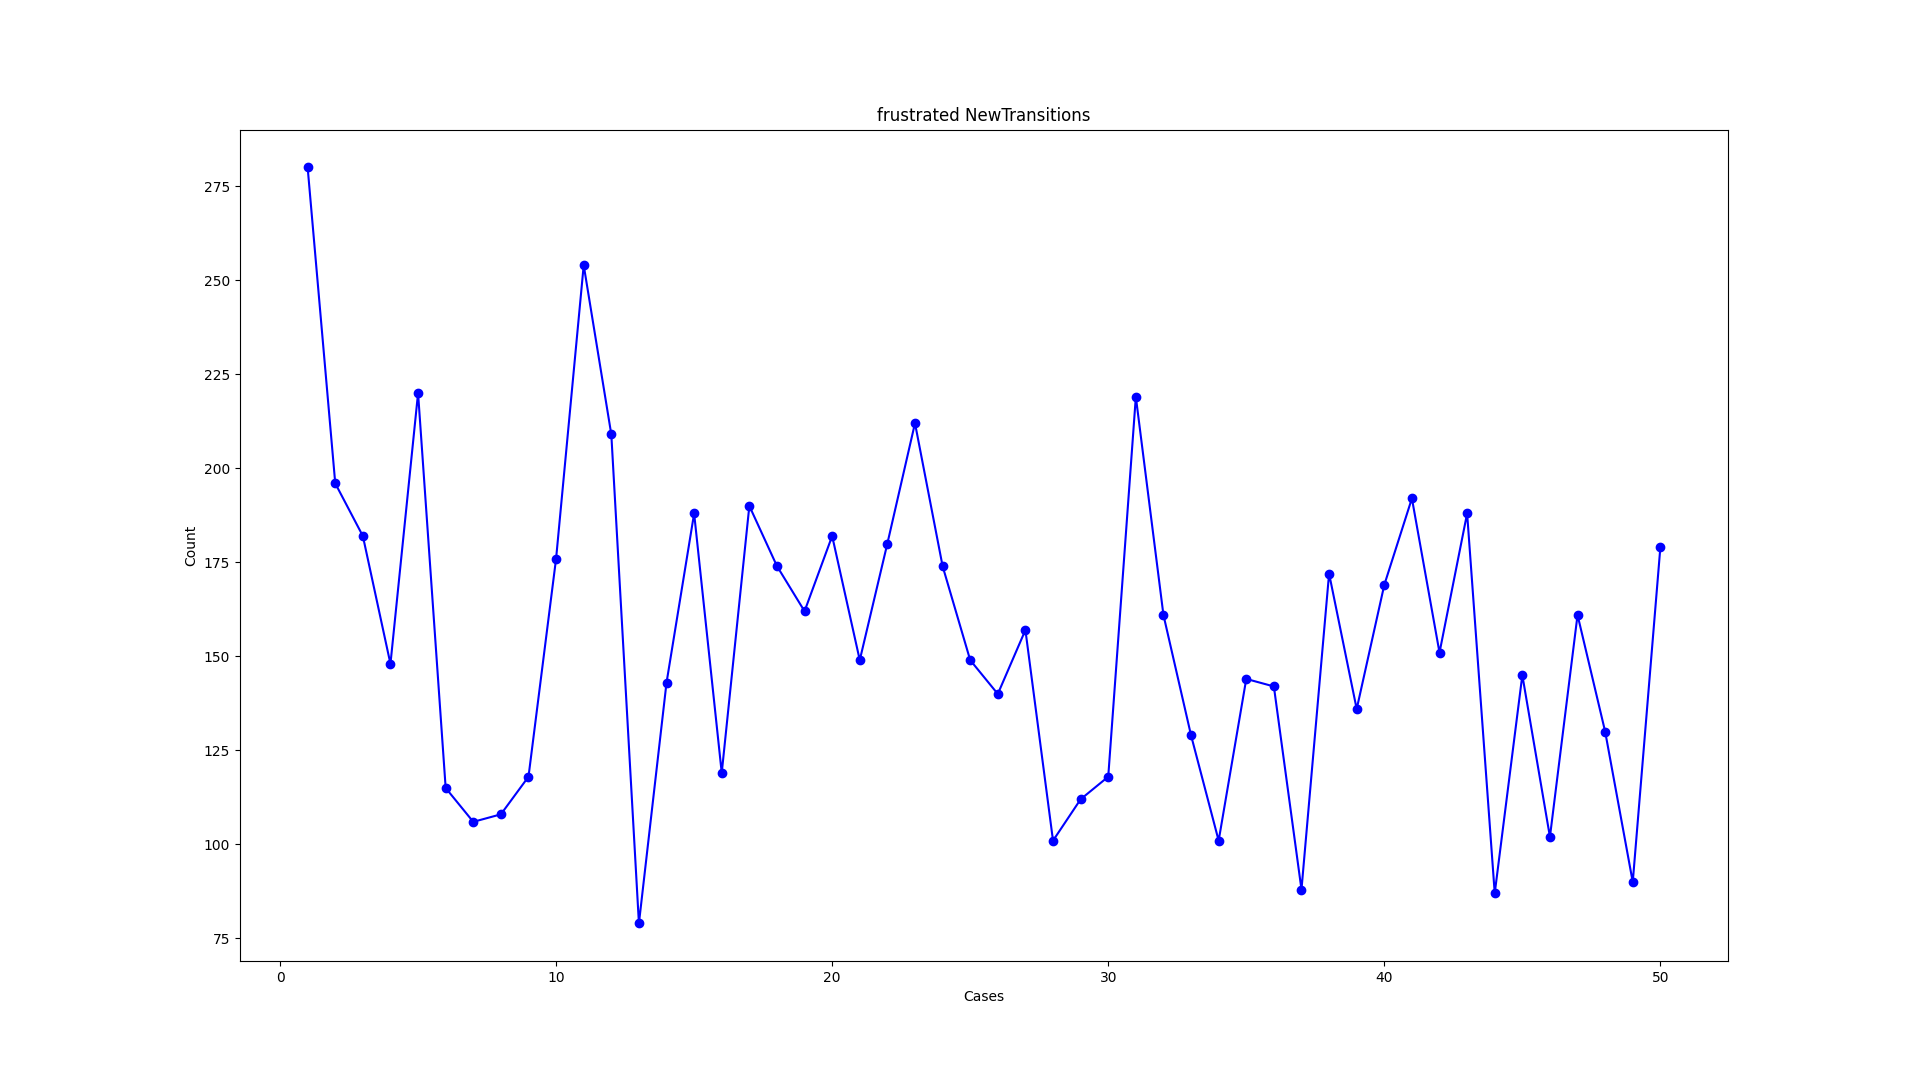
\includegraphics[width=1\linewidth]{images/frustrated NewTransitions.png}
\end{figure}\clearpage

Come è possibile notare dai grafici sopra riportati:

per quanto riguarda le task, dopo pochi video il numero di nuove task trovate scende a 0.

mentre per quanto riguarda le transizioni non c’è una convergenza vera e propria con 50 video ma è presente un accenno di un progressivo abbassamento dei picchi.

Vengono in mente più possibili soluzioni da provare per risolvere questa problematica:
\begin {itemize}
\item cambiare dataset per ottenerne un altro che contenga dei video nei quali sono presenti solo frame molto specifici in relazione al singolo mood e non anche frame che presentano altre espressioni facciali (che comunque sfociano nel mood categorizzato) come in DAiSEE.
Per fare questo, oltre a trovare un altro dataset con questi dati, si potrebbe, con l’aiuto di un esperto, tagliare i video già presenti per ottenere dei video con all’interno solo i frame interessati.
\item un altro approccio potrebbe essere fornire un numero maggiore di dati fino ad arrivare a 0 nuove transizioni; per quanto riguarda questo approccio ho provato a trovare, attraverso la regressione lineare, una linea che descrivesse l’andamento dei vari grafici tracciati utilizzando, sull’asse delle ascisse, il conto delle transizioni e, sull’asse delle ordinate, il numero di transizioni in quel momento (quindi come nei grafici riportati sopra).

Ho trovato la linea sopracitata e ho generato anche i valori successivi fino ad arrivare al primo valore pari o minore a 0. 

Essendo stato rilevato dal metodo utilizzando un trend negativo non sono presenti valori maggiori di 0 dopo il primo valore minore o uguale a 0.

Il numero di passaggi successivi calcolato è riportato nell’immagine qui sotto:
\begin{figure}
    \begin{center}    
        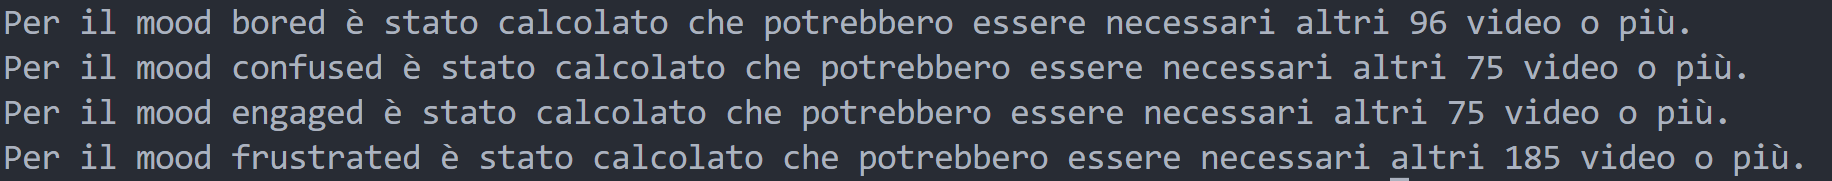
\includegraphics[width=1\linewidth]{images/passaggi aggiuntivi.png}
    \end{center}
\end{figure}
Qui invece riporto i grafici generati con i nuovi possibili valori trovati:
\begin{figure}
    \begin{center}    
        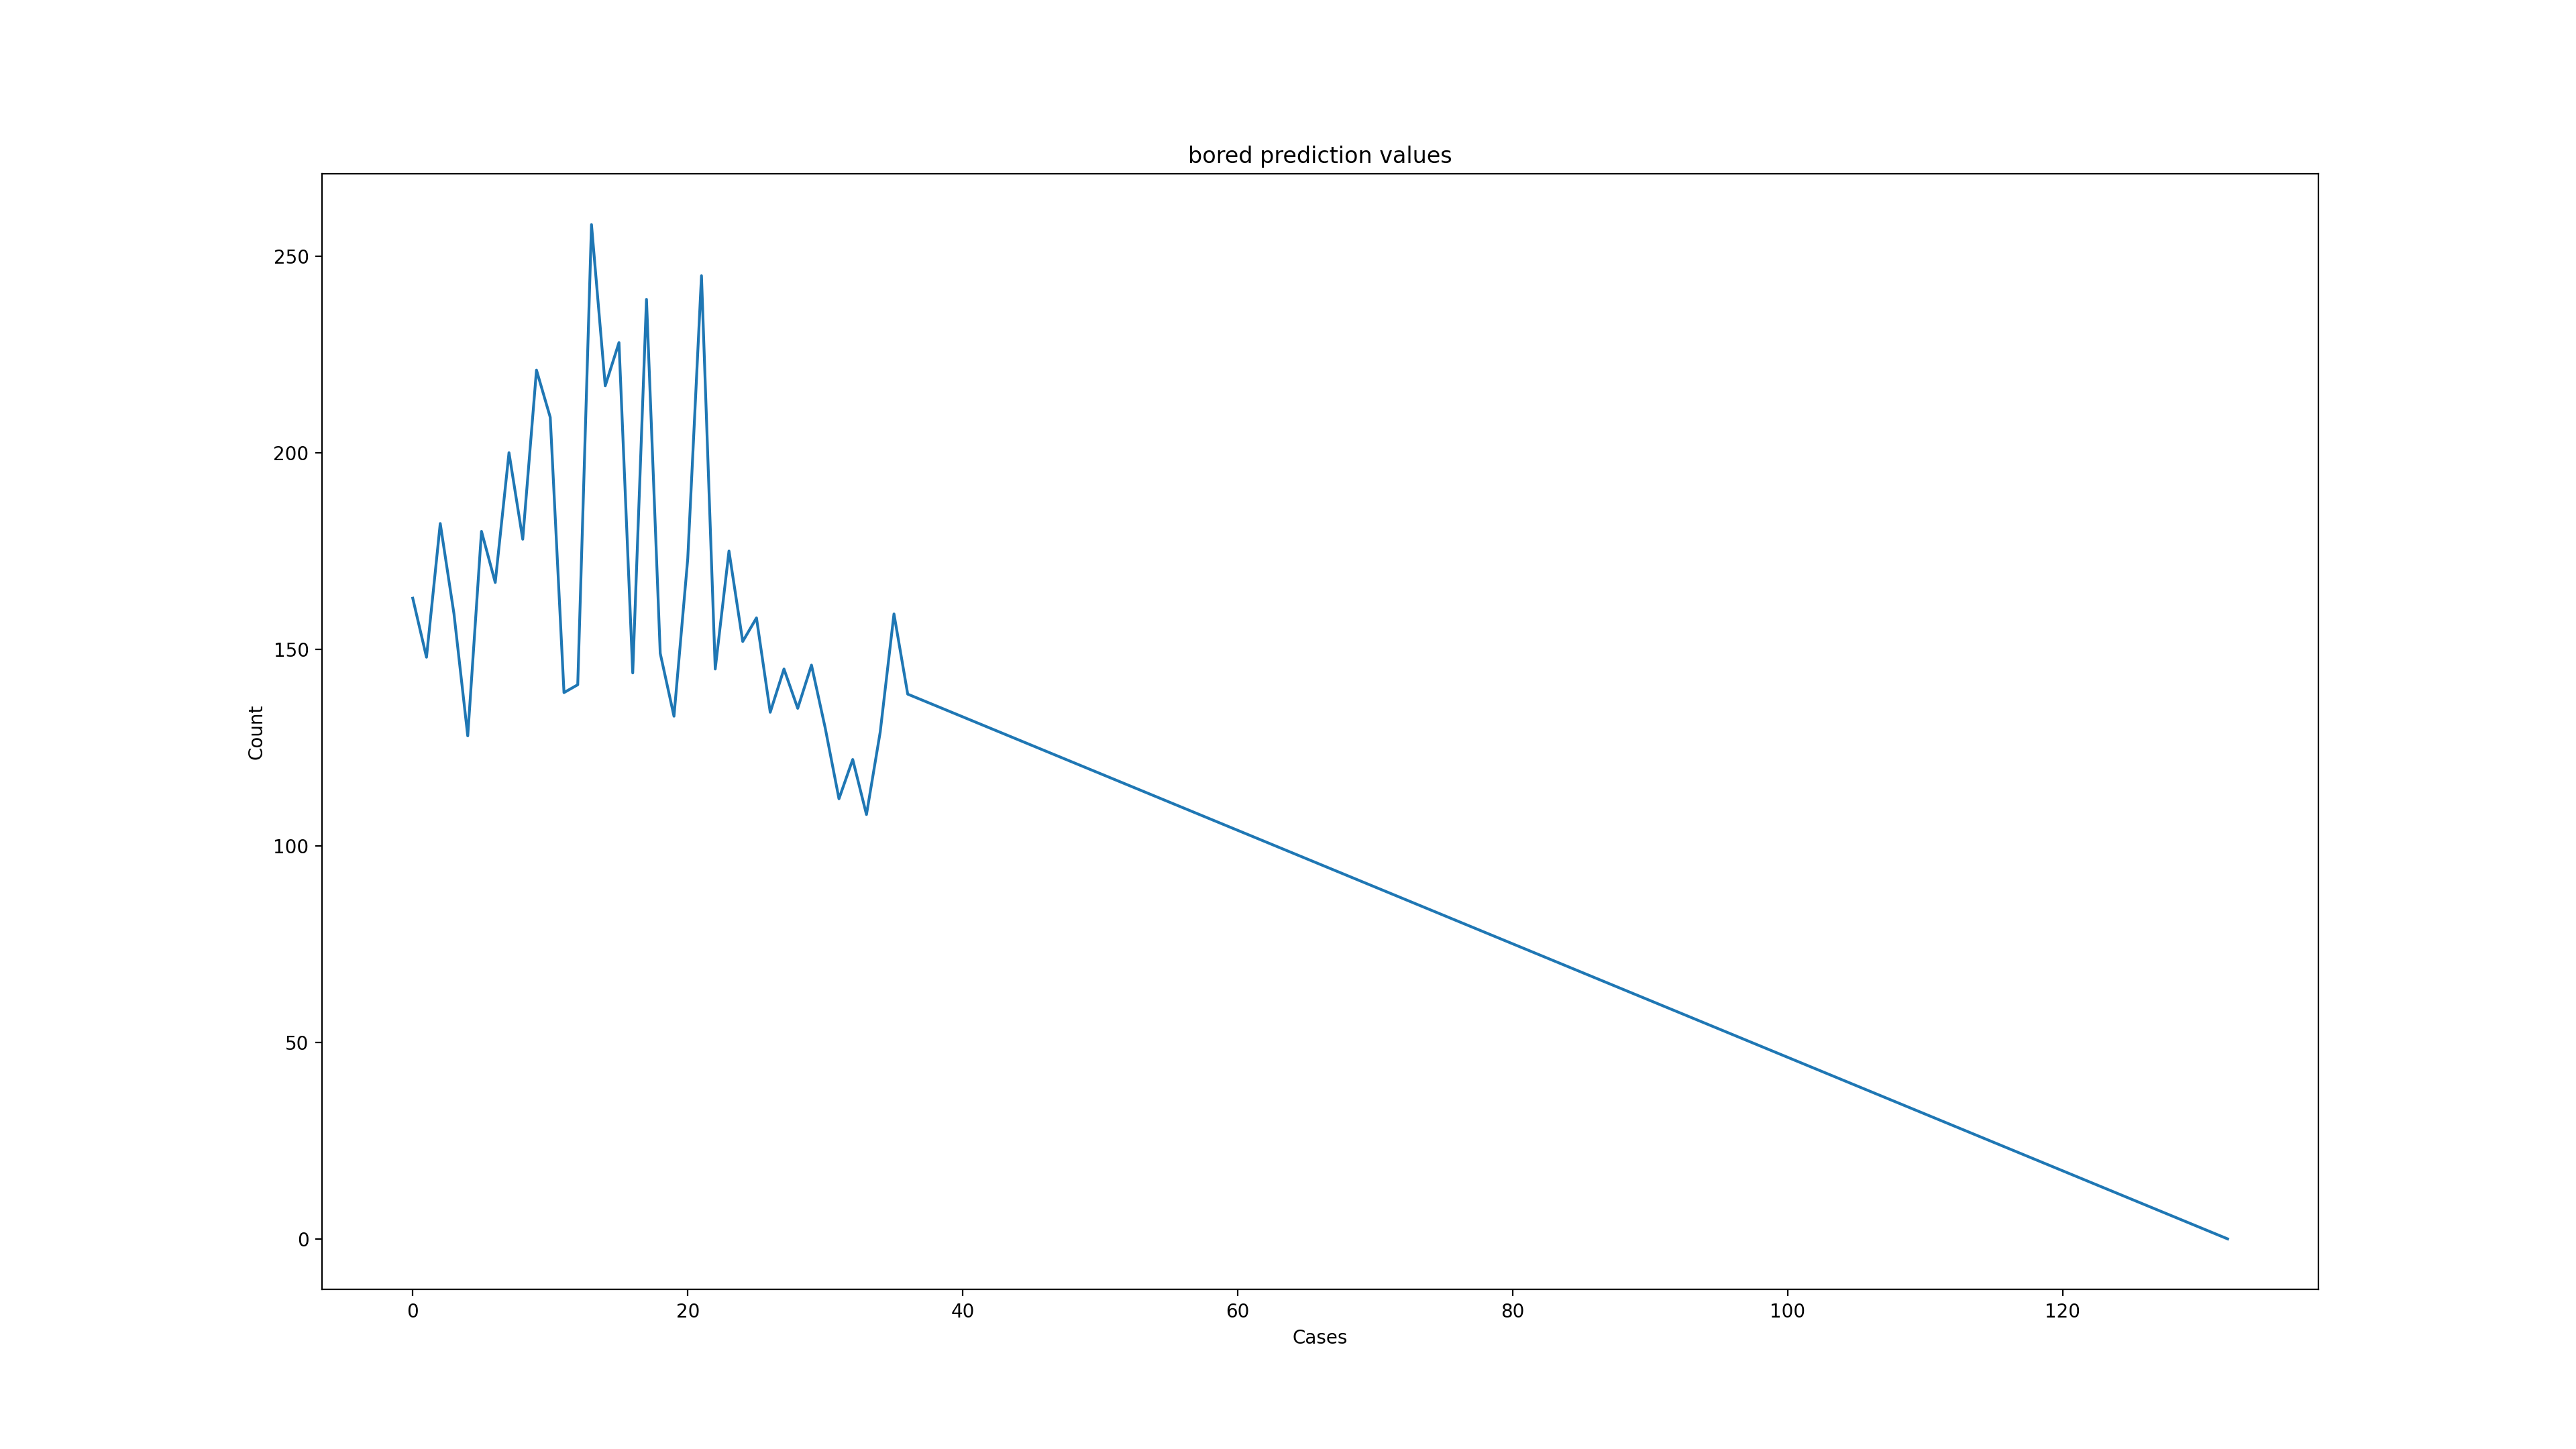
\includegraphics[width=1\linewidth]{images/bored prediction values.png}
    \end{center}
\end{figure}
\begin{figure}
    \begin{center}    
        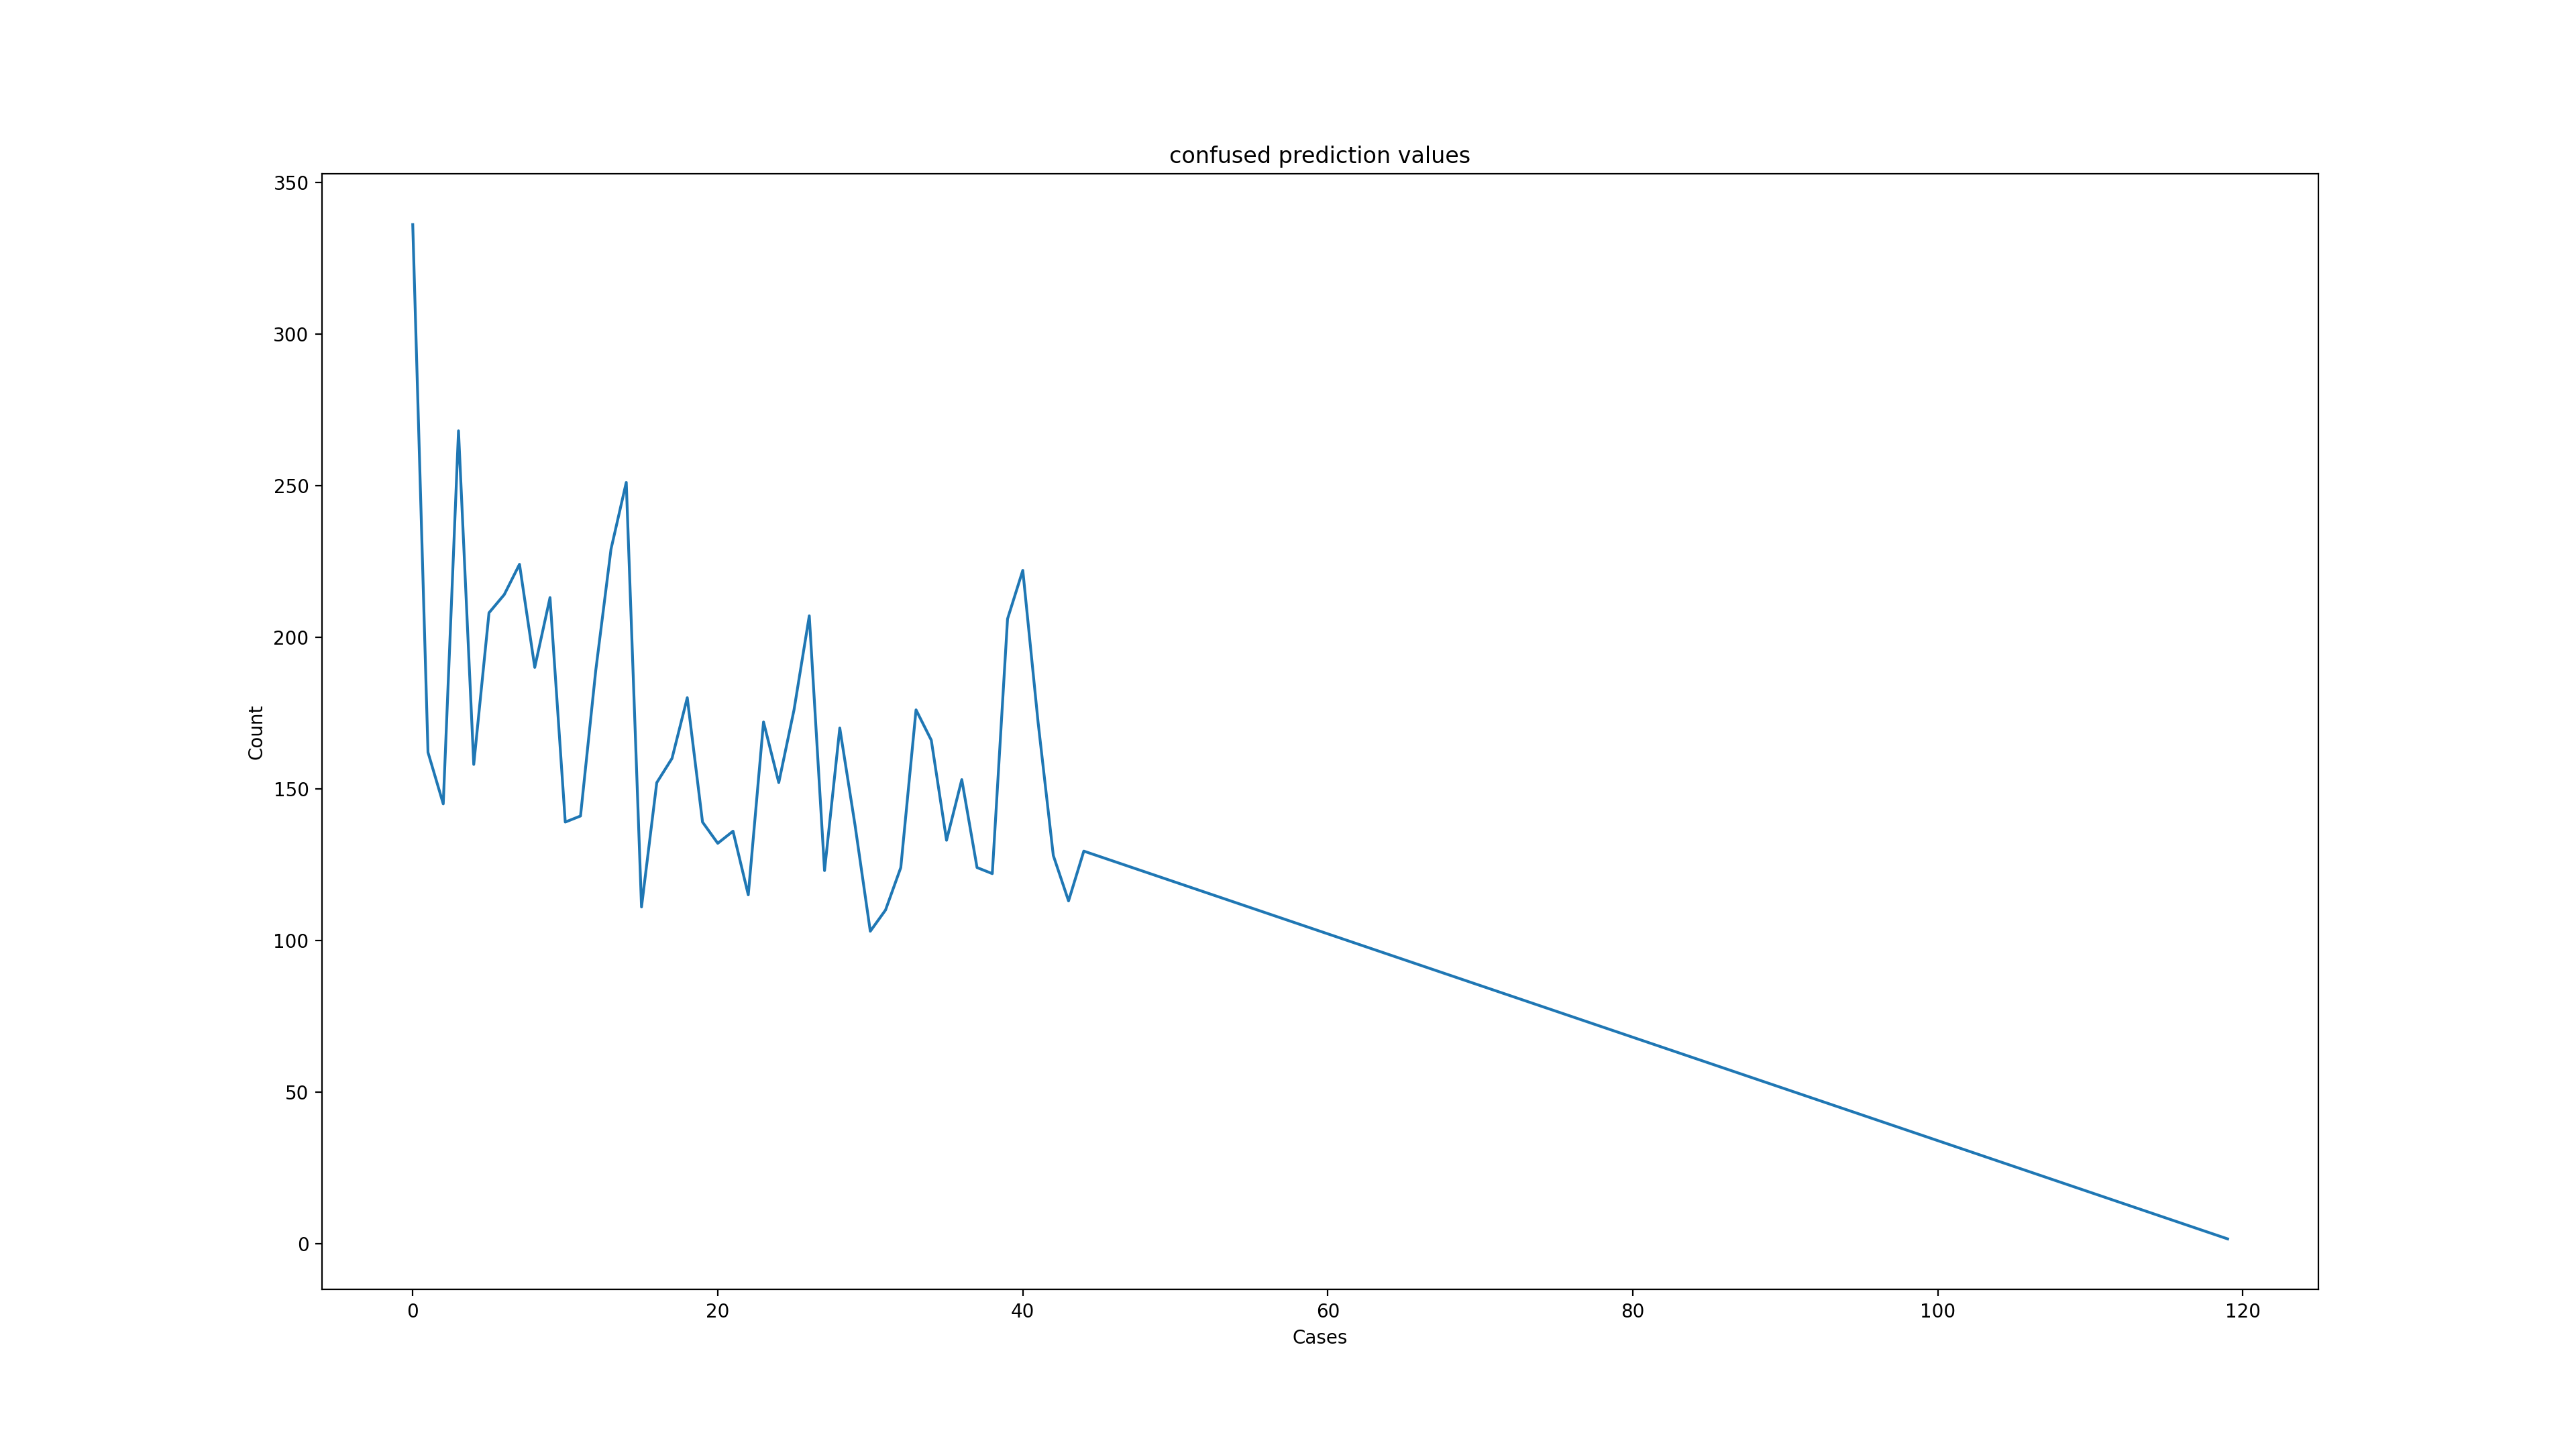
\includegraphics[width=1\linewidth]{images/confused prediction values.png}
    \end{center}
\end{figure}\clearpage
\begin{figure}
    \begin{center}    
        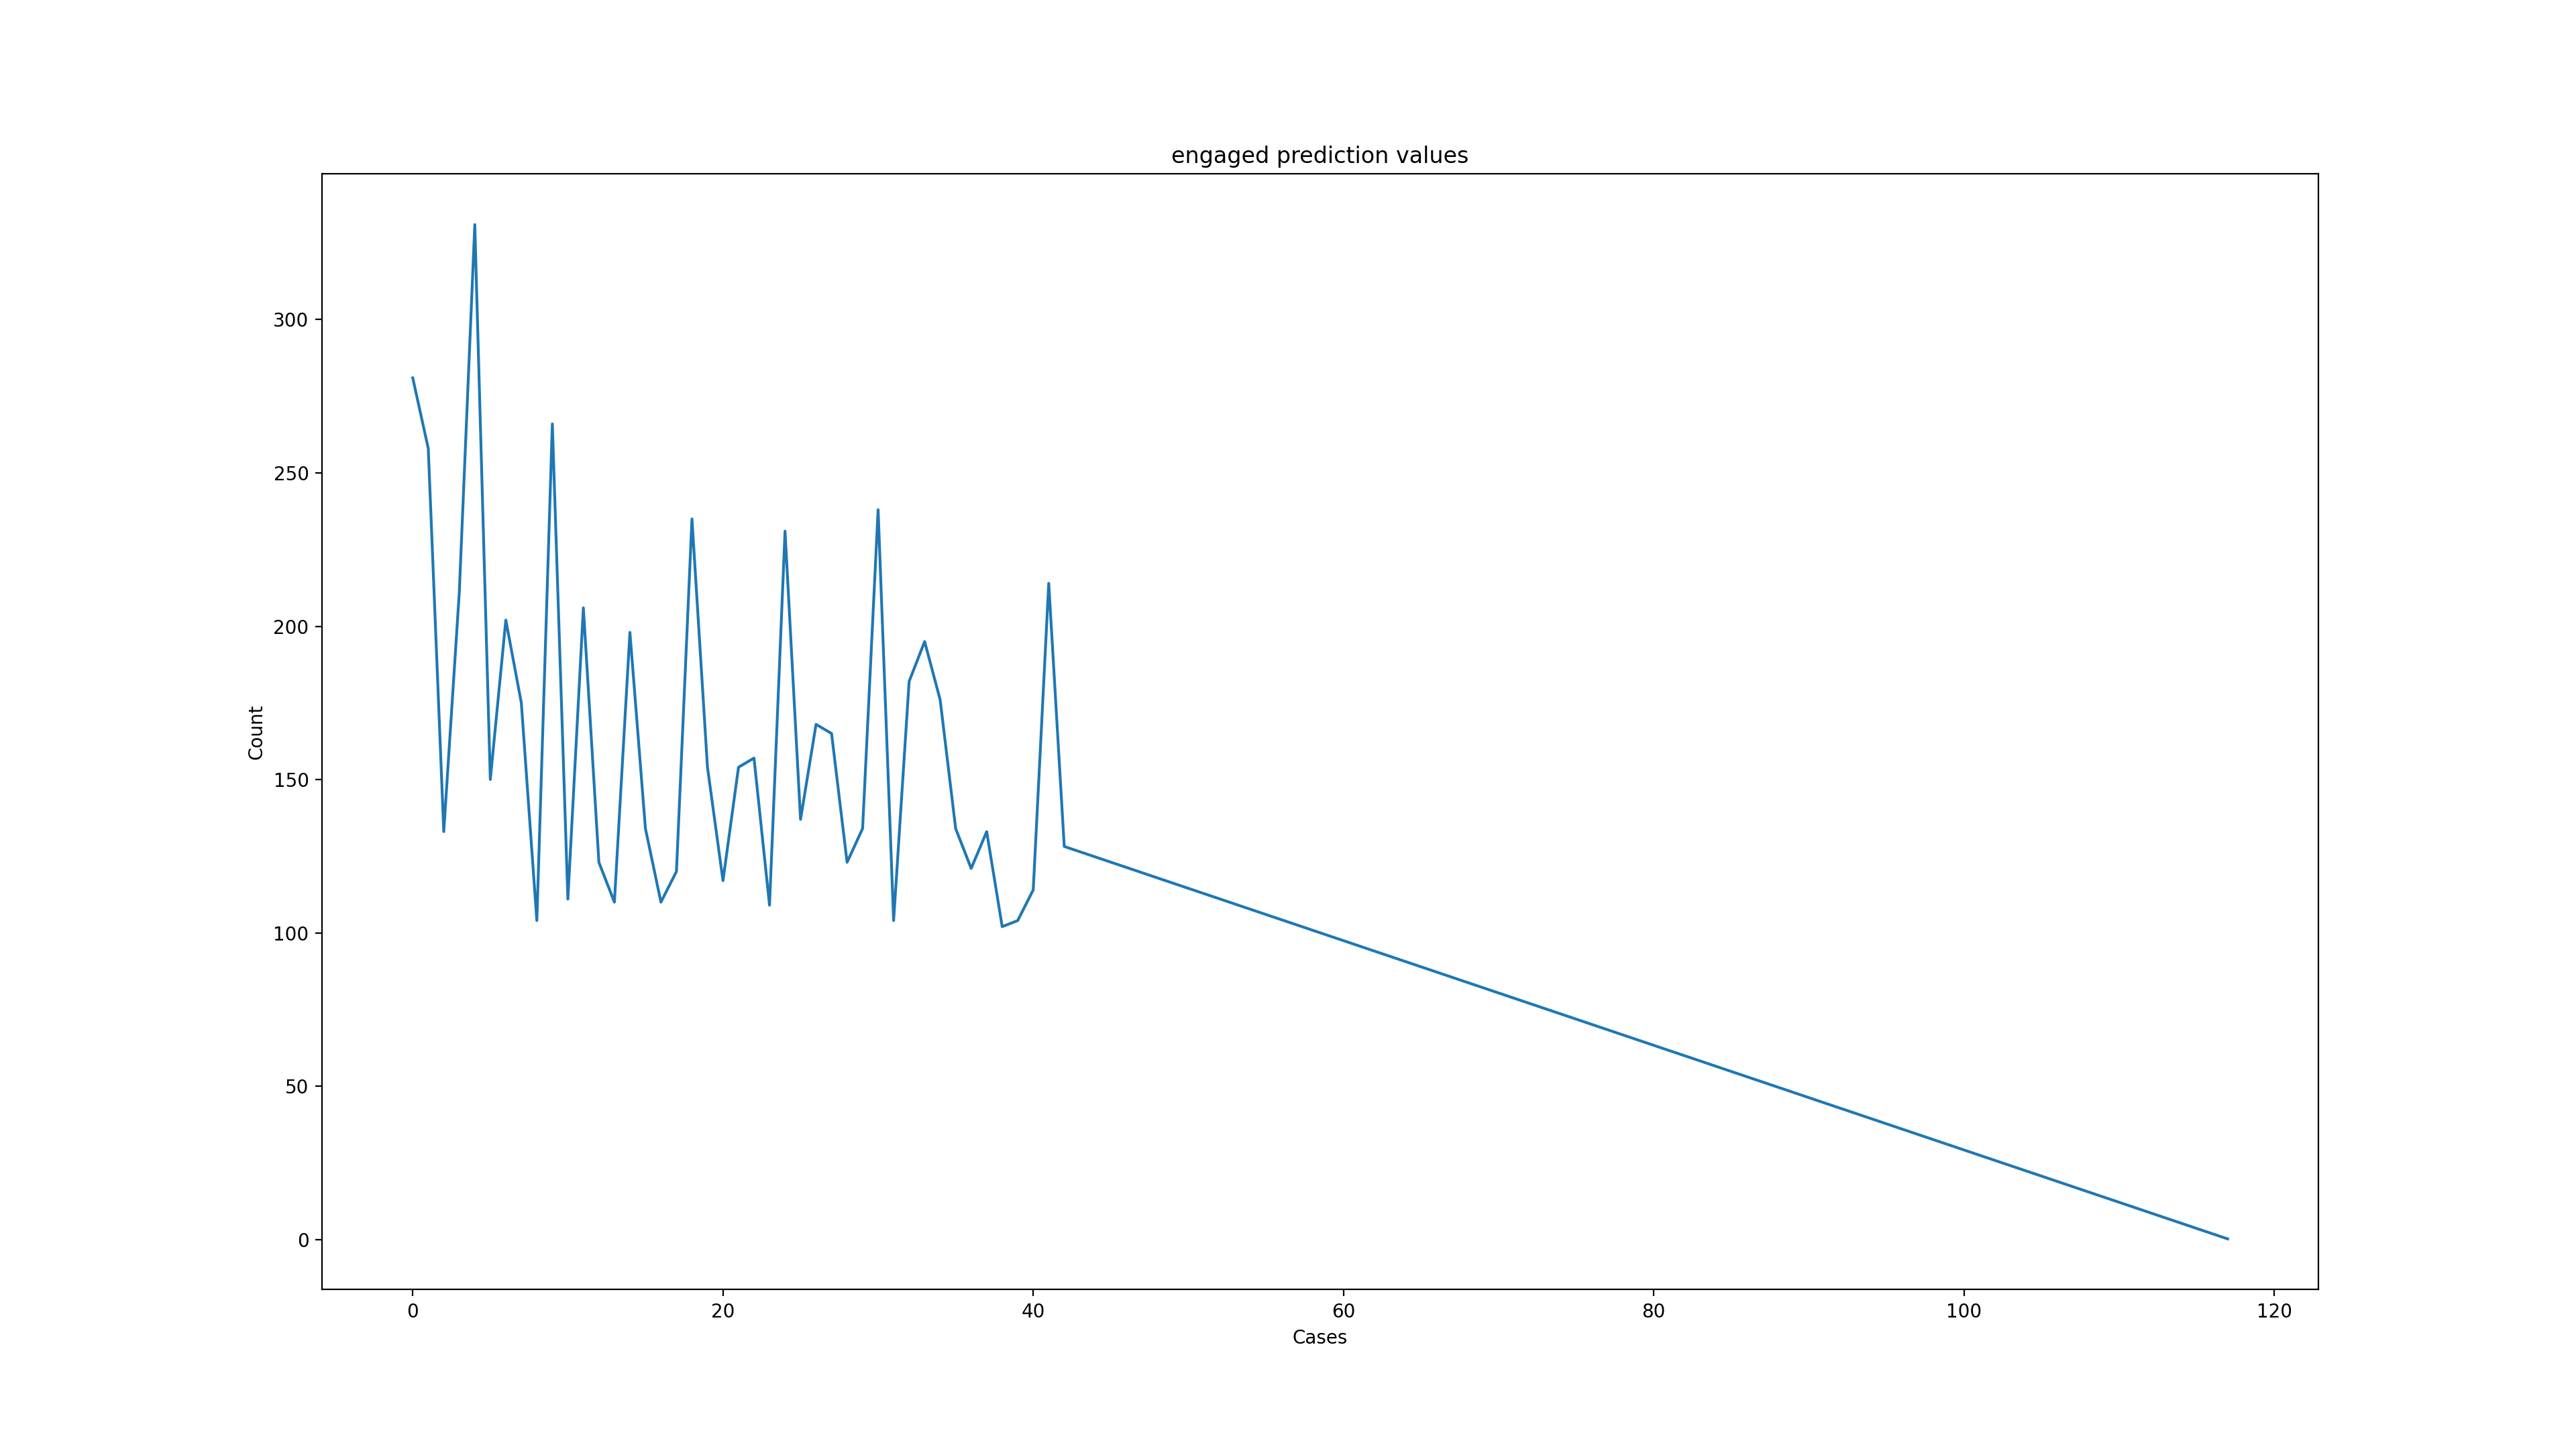
\includegraphics[width=1\linewidth]{images/engaged prediction values.png}
    \end{center}
\end{figure}
\begin{figure}
    \begin{center}    
        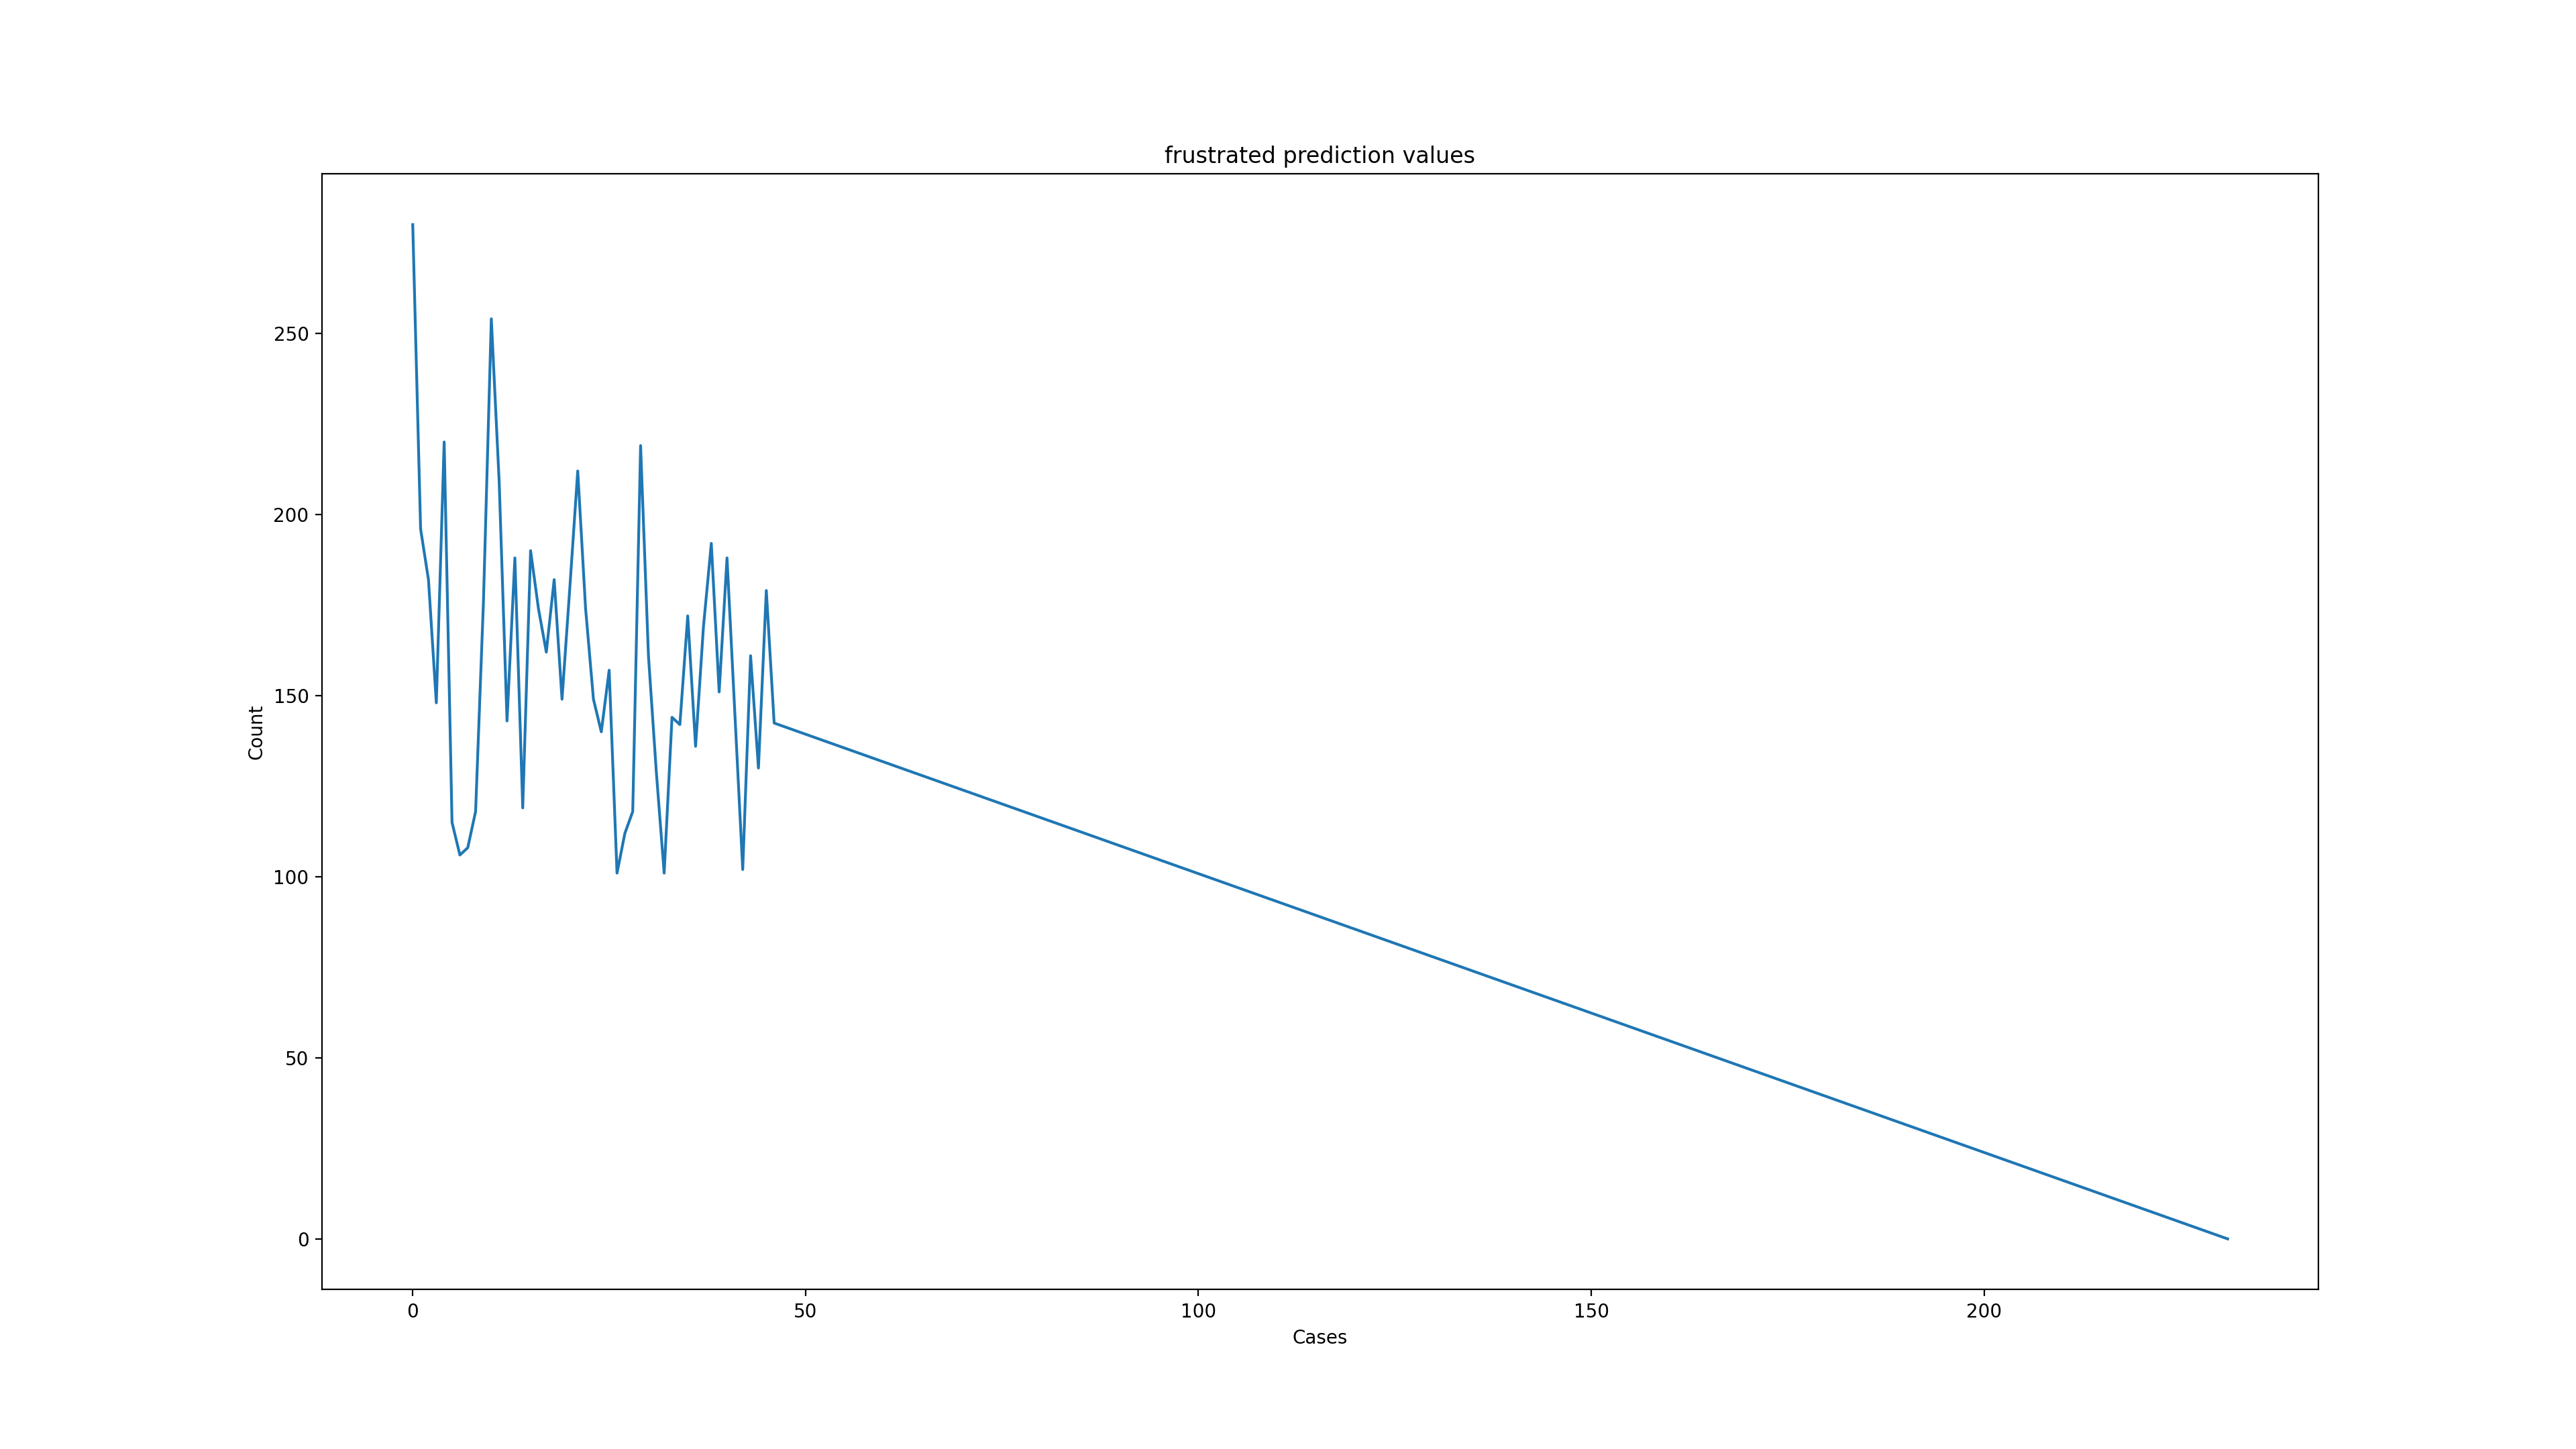
\includegraphics[width=1\linewidth]{images/frustrated prediction values.png}
    \end{center}
\end{figure}\clearpage
\end{itemize}
\newpage

Dalla seconda categoria di file con i modelli generati per ogni mood e dai file da me generati con all’interno le estrazioni create dai video ho estratto invece i seguenti dati:


\begin{table}
    \small
    \centering
    \begin{tabular}{|c|p{2.8cm}|p{2.8cm}|p{2.8cm}|p{2.8cm}|}
        \hline
        Mood       &   Numero di \newline attività &   Numero di eventi &   Numero di task &   Numero di \newline transizioni \\
        \hline
        bored      &                 50 &          33103 &            50 &                7051 \\
        \hline
        confused   &                 50 &          36350 &            50 &                7905 \\
        \hline
        engaged    &                 50 &          36601 &            50 &                7624 \\
        \hline
        frustrated &                 50 &          33407 &            50 &                7727 \\
        \hline
    \end{tabular}
\end{table}

